\pdfinfoomitdate=1
\pdftrailerid{}
\pdfsuppressptexinfo=15
\documentclass[11pt]{article}
\usepackage[margin=1in]{geometry}
\usepackage[T1]{fontenc}
\usepackage{lmodern}
\usepackage{amsmath,amssymb,amsthm,mathtools}
\usepackage{microtype}
\usepackage{needspace}
\usepackage{enumitem,booktabs,array}
\usepackage[numbers,sort&compress]{natbib}
\usepackage{xurl}
\usepackage[dvipsnames]{xcolor}
\usepackage{tikz}
\usetikzlibrary{arrows.meta,positioning,calc,fit,patterns}
\usepackage[colorlinks=true,linkcolor=MidnightBlue,citecolor=MidnightBlue,urlcolor=MidnightBlue]{hyperref}
\newcommand{\R}{\mathbb R}
\DeclareMathOperator{\conv}{conv}
\DeclareMathOperator{\Ent}{Ent}
\DeclareMathOperator{\rank}{rank}
\DeclareMathOperator{\tr}{tr}
\DeclareMathOperator{\supp}{supp}
\DeclareMathOperator{\Cov}{Cov}
\DeclareMathOperator{\Var}{Var}
\DeclareMathOperator{\diag}{diag}
\DeclareMathOperator{\aff}{aff}
\DeclareMathOperator{\ri}{ri}
\DeclareMathOperator{\poly}{poly}
\newcommand{\E}{\mathbb E}
\setlist{topsep=5pt,itemsep=3pt,parsep=0pt}
\setlength{\emergencystretch}{2em}
\newtheorem{theorem}{Theorem}[section]
\newtheorem{lemma}[theorem]{Lemma}
\newtheorem{proposition}[theorem]{Proposition}
\newtheorem{corollary}[theorem]{Corollary}
\theoremstyle{remark}
\newtheorem{remark}[theorem]{Remark}
\theoremstyle{definition}
\newtheorem{definition}[theorem]{Definition}
\hypersetup{pdftitle={Entropy and Face Dimension of the Perfect-Matching Polytope},pdfauthor={OpenAI}}
\title{Entropy and Face Dimension of the Perfect-Matching Polytope}
\author{OpenAI}
\date{September 23, 2026}
\begin{document}
\maketitle
\begin{abstract}
We prove the perfect-matching entropy conjecture of Anari, Oveis Gharan,
and Vinzant. For every feasible vector $x$ of perfect-matching edge marginals
in a loopless labelled multigraph on $2m\ge2$ vertices, the maximum entropy
$H(x)$ of a matching law with marginals $x$ satisfies
\[
F(x)-(2-2/m)B(x)\le H(x)\le F(x),
\]
where $F(x)=-\sum_e x_e\log x_e$ and
$B(x)=-\sum_e(1-x_e)\log(1-x_e)$.
This bound holds throughout the polytope, including its boundary.
We also prove the sharp bound $|\supp x|-\dim F_x\le3m-2$, where $F_x$ is
the minimal face of the perfect-matching polytope containing $x$.
\end{abstract}
\section{Introduction}

Prescribing the probability that each edge belongs to a random perfect
matching does not prescribe the distribution of the whole matching.
The largest possible entropy of such a distribution measures how many
matching choices can coexist with those edge probabilities. We bound
this entropy by explicit sums of one-coordinate functions, at every
feasible mean. The result yields lower counts from uniform marginals
and additive estimates for weighted partition functions.

Throughout, a graph is finite, undirected and loopless. Parallel edges
are distinguished both as coordinates and as choices in a matching.
A perfect matching covers each vertex by exactly one edge. Write
$\mathcal M(G)$ for the set of perfect matchings,
$N(G)=|\mathcal M(G)|$, and
\[
 P(G)=\conv\{\mathbf1_M:M\in\mathcal M(G)\}\subseteq\R^{E(G)}
\]
for their polytope. Thus a point $x\in P(G)$ is exactly a feasible
vector of edge probabilities. For a probability law $p$ on the matching
family, put $\Ent(p)=-\sum_M p_M\log p_M$, and define
\begin{align}
 H(x)&=\max\left\{\Ent(p):p\text{ is a probability law on }\mathcal M(G),\
                   \sum_Mp_M\mathbf1_M=x\right\},\label{intro:H}\\
 F(x)&=-\sum_{e\in E(G)}x_e\log x_e,\qquad
 B(x)=-\sum_{e\in E(G)}(1-x_e)\log(1-x_e).
 \label{intro:FB}
\end{align}
All unqualified logarithms are natural, and $0\log0=0$.
The maximum in Equation~\eqref{intro:H} is attained by compactness
of the feasible set of laws. No connectedness or bipartiteness is assumed.

\begin{theorem}[Pointwise entropy bounds]\label{ent:main}
Let $G$ be a loopless multigraph on $2m\ge2$ vertices with at least one
perfect matching. For every $x\in P(G)$,
\begin{equation}\label{intro:main-bound}
                  F(x)-\left(2-\frac2m\right)B(x)
                  \le H(x)\le F(x).
\end{equation}
\end{theorem}

In particular, $H\ge F-2B$ throughout the polytope, including its
boundary. When $m=1$, each matching is one of the distinguished edges
between two vertices, and the bounds give the exact identity $H=F$.
For the empty vertex set the unique empty matching gives $F=B=H=0$;
the formula involving $1/m$ is not used.

The upper bound $H\le F$ is a direct instance of Shearer's entropy
inequality~\citep{ChungGrahamFranklShearer1986}: each edge occurs in
two vertex stars, and a matching chooses exactly one edge at each
vertex. Our contribution to Equation~\eqref{intro:main-bound} is its
lower comparison. The coefficient there is obtained from a geometric
rank estimate followed by a covariance calculation, with no assumption
that the mean is interior to the full polytope.

Edmonds' matching-polytope theorem~\citep{Edmonds1965} describes feasible
matching means by degree equations, nonnegativity and odd-cut
inequalities. The odd cuts distinguish general graphs from bipartite
graphs and are also central to the entropy bound here. Bipartite graphs
admit an order-independent coefficient-one comparison:
Schrijver's inequality~\citep{Schrijver1998Counting} and the weighted Bethe
inequality of Gurvits~\citep[expanded version, Theorem~2.2]{Gurvits2011SchrijverBethe}, together with
entropy duality, imply $H(x)\ge F(x)-B(x)$. Their permanent setting is
essential to this comparison. In Section~\ref{ex:sec-triangle-expansions} we give a
simple eight-vertex nonbipartite graph with a feasible mean for which
$H<F-B$.

\subsection{Entropy and structural consequences}

Anari, Oveis Gharan and Vinzant~\citep[FOCS version, Conjecture~6]{AnariOveisGharanVinzant2018}
proposed a convex-optimization framework for approximate counting
and asked whether the maximum binary-coordinate entropy of a perfect
matching mean exceeds $\log N(G)$ by only a linear function of the
number of vertices. In our notation their objective is $F+B$.
Theorem~\ref{ent:main} gives the explicit positive answer
\[
 \log N(G)\le\max_{x\in P(G)}(F(x)+B(x))
                       \le\log N(G)+3m-2.
\]
The pointwise statement also controls arbitrary finite edge weights,
through the Gibbs variational formula. The proposed linear-error
estimate is therefore an optimized consequence of the prescribed-mean
inequality, rather than its definition. Corollary~\ref{cons:entropy-count} proves the optimized bounds, and
Section~\ref{cons:weighted-section} derives the weighted form.

If $G$ contains $k\ge2$ edge-disjoint perfect matchings, their uniform
mixture has marginal $1/k$ on their union. Substituting that mean into
Theorem~\ref{ent:main} gives
\[
 N(G)\ge k^m(1-1/k)^{2(m-1)(k-1)}
       \ge e^{-2(m-1)}k^m.
\]
The same estimate holds for a $k$-regular graph whose every odd cut has
at least $k$ edges, because its uniform vector belongs to $P(G)$.
These consequences and their endpoint cases are proved in
Section~\ref{cons:section}.

For structural counts, the scale of the degree matters. Esperet,
Kardo\v{s}, King, Kr\'a\v{l} and Norine~\citep{EsperetEtAl2011}
proved an exponential lower bound for every bridgeless cubic graph.
Abdi, Cornu\'ejols, Dadush and Dalirrooyfard~\citep[Corollary~6.6]{AbdiCornuejolsDadushDalirrooyfard2026}
proved exponential lower bounds for all regular graphs of degree at
least four satisfying the corresponding odd-cut condition, including
matchings crossing every minimum odd cut exactly once.
Ebrahimnejad, Nagda and Oveis Gharan~\citep{EbrahimnejadEtAl2021}
gave quantitative lower counts for regular nonbipartite graphs under
an additional spectral-expansion hypothesis. The estimate
$(k/e^2)^m$ obtained here has a base growing with the degree $k$.
At small fixed degree these earlier exponential results can be
stronger: our displayed homogeneous base is greater than one only
when $k\ge8$. On the bipartite subclass Schrijver's bound has the
stronger asymptotic base $k/e$ per matched pair. Our structural
statements concern the explicit odd-cut condition; merely requiring
every edge to belong to a perfect matching is a different hypothesis.
Esperet et al. formulate the growing-degree question on the broader
matching-covered class \citep[corrected full version, Conjecture~24]{EsperetEtAl2011}.
Our regular odd-cut corollary also establishes the even-order connectivity
formulation of \citet[arXiv version, Conjecture~1.1]{EbrahimnejadEtAl2021}.\footnote{The
cited arXiv version writes the degree as $d$ but prints an undeclared
$k-1$ in the connectivity condition. We read it as $d-1$, consistently
with its Section~1.2.}

\subsection{Face dimension and the entropy argument}

For a graph on $2m\ge2$ vertices and $x\in P(G)$, let $F_x$ be its
minimal face, the smallest face of
$P(G)$ containing $x$, and let $\supp x=\{e:x_e>0\}$.
The geometric input is the sharp estimate
\[
                  |\supp x|-\dim F_x\le3m-2.
\]
Edmonds' theorem identifies the left side with the rank of the tight
odd-cut equations on the supported coordinates; singleton cuts supply
the degree equations. Abdi et al.~\citep[Lemmas~6.4--6.5]{AbdiCornuejolsDadushDalirrooyfard2026}
bound this rank by $3m-1$ using odd laminar families.
Their cubic staircase examples already have minimum-odd-cut rank
$|E|-2$, attaining $3m-2$
\citep[discussion after Corollary~6.6 and Figure~2]{AbdiCornuejolsDadushDalirrooyfard2026}.

The dimension of the whole perfect-matching polytope was characterized
by Naddef~\citep{Naddef1982} and by Edmonds, Pulleyblank and
Lov\'asz~\citep{EdmondsPulleyblankLovasz1982}, whose brick decomposition
uses cuts crossed once by every perfect matching. Here a cut need only
be tight at the prescribed mean: it is crossed once by every matching
in that minimal face, but possibly not by every matching of the graph.
Section~\ref{geom:sec-polytope} proves the supported bound by contracting
such a cut. A direction in the parent face can be assembled from
directions in the two contracted faces when their crossing-edge
coordinates agree. Each crossing-coordinate sum is zero, by the degree
equation at the contracted vertex. Agreement therefore imposes at most
$|C|-1$ independent conditions for a cut $C$, rather than $|C|$.
This saved condition closes an induction with bound $3m-2$.
Appendix~\ref{a:section} also gives the laminar proof. It uses the standard
face-restricted uncrossing argument
\citep[full version, Lemma~2.2 and Appendix~A]{SvenssonTarnawski2017}
and retains the dependence between complementary root children in the
laminar tree.

The analytic step uses the classical exponential form of a
maximum-entropy law under mean constraints
\citep{Jaynes1957,SinghVishnoi2014}. Its log-partition Hessian is the
covariance matrix, as in standard exponential-family theory
\citep{WainwrightJordan2008}. We restrict the law to the atoms of $F_x$.
Its covariance then has image equal to the direction space of that face,
even when it is singular in the ambient edge space.

Suppose that $F-cB-H$ has a positive maximum. Removing coordinates fixed
at zero or one leaves strictly fractional means and preserves this
entropy deficit. Exponential tilts within the resulting minimal face
supply smooth curves through the maximum. First-order stationarity
cancels the acceleration term in their second derivatives. Summing the
second-derivative inequalities over positive covariance eigenvalues
bounds the face dimension above, contradicting the geometric lower bound
whenever $c>2-2/m$ for the original graph. Passing to the endpoint proves
Theorem~\ref{ent:main}. Section~\ref{sec:entropy} carries this out within
the face, without inverting an ambient covariance kernel or differentiating
across faces.

Section~\ref{ex:sec-triangle-expansions} explains both geometric sharpness
and the obstruction to coefficient one. We use the triangle expansions
underlying the Klee graphs of
Cygan, Pilipczuk and \v{S}krekovski~\citep{CyganPilipczukSkrekovski2013}
to construct a two-dimensional minimal face on every positive even
order. At uniform edge marginals, a matching law is forced onto its
three vertices even when the graph has further matchings. These examples
attain the geometric bound and give the coefficient-one counterexample;
they do not establish optimality of the coefficient two.

\subsection{Deterministic counting with binary multiplicities}

For the algorithmic problem, the input specifies a vertex set and
nonnegative integer multiplicities $k_{ij}$ in binary for unordered pairs
of distinct vertices; omitted pairs have multiplicity zero. Its count is
\[
 N(G)=\sum_M\prod_{\{i,j\}\in M} k_{ij},
\]
where $M$ runs over pairings of the vertex set. The input can also list
parallel edges explicitly. The algorithm uses the binary multiplicities
without expanding them into labelled copies.

\begin{theorem}[Deterministic approximate counting]
\label{thm:main}\label{thm:algorithm-guarantee}
There is one uniform deterministic algorithm which, on a graph on $n$
vertices with nonnegative binary integer pair multiplicities, returns an
integer $A\ge0$ satisfying
\[
                         N(G)/512^n\le A\le N(G).
\]
Its running time and output length are polynomial in the input bit length.
In particular, $A=0$ exactly when $N(G)=0$. The guarantee includes a compact
input consisting of binary $n$ and a list of positive pair records.
\end{theorem}

The factor $512^n$ permits a complete implementation with integer and
rational arithmetic and a fixed polynomial number of steps. The degree
of this polynomial is large; the theorem gives a complexity guarantee,
not a practical running-time benchmark. Appendix~\ref{c:app-loops} treats
the different convention that a loop covers its one incident vertex. It
returns a rational approximation within factor $2^{18n}$, including when
the original vertex count is odd.

\paragraph{Approximation history and computational models.}

Exact counting is $\#\mathrm P$-complete even for bipartite perfect
matchings, through the permanent of a zero--one matrix
\citep[Theorem~1]{Valiant1979}. For an $r\times r$ nonnegative matrix,
Linial, Samorodnitsky and Wigderson give an $e^r$-factor deterministic
strongly polynomial arithmetic algorithm
\citep[author version, Theorem~1.1]{LinialSamorodnitskyWigderson2000}.
Jerrum, Sinclair and Vigoda give a fully polynomial randomized
approximation scheme for the nonnegative permanent
\citep{JerrumSinclairVigoda2004}. For nonnegative rational matrices, Kudria, Luo and Majid give certified
rational endpoints in polynomial bit time with logarithmic width
$O(r(\log\log r)^2/\log r)$
\citep[Theorem~1.1]{KudriaLuoMajid2026}, while Dong and Jain give factor
$(1+\varepsilon)^r$ for every fixed $0<\varepsilon\le1$ in a strongly
polynomial arithmetic model
\citep[Theorem~1.1 and Section~1.1]{DongJain2026}.
These permanent results concern bipartite graphs on $2r$ vertices.

The analogous function for a general graph is the \emph{hafnian}: the
sum of products over pairings of the indices of a symmetric matrix.
Barvinok describes a randomized exponential-factor approximation for
nonnegative hafnians \citep[author preprint, Section~7]{Barvinok1999}.
For fixed $\delta>0$ and any $0<\varepsilon<1$, his later theorem approximates
$\ln\operatorname{haf}(A)$ to additive error $\varepsilon$ using
$r^{O_\delta(\log r+\log(1/\varepsilon))}$ arithmetic operations when the entries of the
symmetric $2r\times2r$ matrix lie in $[\delta,1]$
\citep[Theorem~2.1]{Barvinok2017}. The diagonal may be filled arbitrarily
in this interval, since a hafnian uses no diagonal entry.
Yi gives a deterministic fully polynomial approximation scheme for
rational hafnian inputs of even order, with zero diagonal, when nonzero
entries lie in $[\theta,1]$ and the support has minimum degree at least
$(1/2+\gamma)$ times its order, for fixed $0<\theta\le1$ and
$0<\gamma<1/2$ \citep[Theorem~1.1(a)]{Yi2026}. These hypotheses differ from arbitrary supports and binary
multiplicities in Theorem~\ref{thm:main}. A separate manuscript treats
fully polynomial randomized relative approximation for arbitrary simple
graphs \citep[Theorem~1.1]{OpenAIMatchingFPRAS2026}.

The construction follows the entropy-optimization approach of
Anari, Oveis Gharan and Vinzant~\citep[FOCS version, Section~I.D]{AnariOveisGharanVinzant2018},
with a rational optimizer and all bit bounds given explicitly here.
Section~\ref{cons:weighted-section} establishes the binary-log weighted
interface. Sections~\ref{d:sec-objective} and~\ref{d:sec-optimization}
first complete the input to $K_n$, assigning tiny positive dyadic
weights to absent pairs. This keeps the optimization polytope nonempty
and separates zero from positive original counts. They then replace
the weighted entropy objective by an integer-slope dyadic interpolant
and an exact penalty on a box. On $K_n$, correcting degrees and then
mixing with the uniform feasible point repairs constraint violations. The resulting fixed-grid
iteration needs only an active violated row. Section~\ref{d:sec-odd-cuts}
finds that row by a parity-preserving cut recursion, and
Section~\ref{d:sec-algorithm} proves the count, zero-detection and
bit-complexity guarantees. Minimum odd cuts as matching-constraint
separators go back to Padberg and Rao~\citep{PadbergRao1982}.
The exponential matching laws used in the entropy proof remain analytic
objects; this algorithm does not query them.

The appendices retain alternative relations between face geometry and
entropy. Appendix~\ref{a:section} gives the laminar and quotient-map
arguments, then the direct coefficient-three and coefficient-four
covariance comparisons and their counting consequences.
Appendix~\ref{b:section} proves the nonlinear entropy-defect bound by
normalizing positive marginals and taking the inverse covariance on
the face's direction space; Appendix~\ref{a:section} also gives its
short scalar deduction. Appendix~\ref{c:app-loops} proves the
singleton-loop reduction and its rational bit complexity.

\section{Faces and tight cuts of the perfect matching polytope}
\label{geom:sec-polytope}

The geometric input to the entropy argument is a bound on the number
of independent equations defining a face on its positive coordinates.
We prove the odd-cut description by gluing matching laws across a tight
cut. The same gluing operation then combines directions in the two
contracted polytopes. Both directions preserve the total mass on the cut,
which saves one compatibility equation and yields the sharp bound
$3m-2$. The laminar proof of the same estimate is given in
Appendix~\ref{a:section}.

Throughout this section, \(G=(V,E)\) is a finite undirected loopless
multigraph of even order \(|V|=2m\). Parallel edges have distinct
labels and coordinates. Write \(\mathcal M(G)\) for its perfect
matchings, put \(a(M)=\mathbf 1_M\in\{0,1\}^{E}\), and define
\[
 P(G)=\operatorname{conv}\{a(M):M\in\mathcal M(G)\}.
\]
The convex hull of an empty matching family is empty. If \(V\) is
empty, its unique perfect matching is the empty matching and its
polytope is a singleton in \(\mathbb R^\varnothing\).
For \(S\subseteq V\), let \(\delta(S)\) be the set of edges with
exactly one endpoint in \(S\), and put
\(\chi_S=\mathbf 1_{\delta(S)}\).
We abbreviate \(\delta(\{v\})\) to \(\delta(v)\), and write
\(x(A)=\sum_{e\in A}x_e\) for \(A\subseteq E\).

\subsection{Contraction and the odd-cut description}

For an odd set $S\subsetneq V$, form $G_1$ by retaining $S$ and
contracting $\overline S=V\setminus S$ to a new vertex, discarding edges
internal to $\overline S$. Form $G_2$ by interchanging the two sides.
Every edge of $C=\delta(S)$ keeps its original label in both graphs;
edges that become parallel are not identified. We call the cut
\emph{nontrivial} when both sides have at least three vertices. In that
case the contracted graphs have smaller even orders.

\begin{lemma}[Gluing across an odd cut]
\label{geom:lem-gluing}\label{a:lem-tight-cut-gluing}
Suppose $y_i\in P(G_i)$, for $i=1,2$, and their coordinates agree on
$C$. There is a point $y\in P(G)$ with the internal coordinates of the
two $y_i$ and their common crossing coordinates.
\end{lemma}

\begin{proof}
Choose a matching law of mean $y_i$ in each contracted graph.
A matching uses exactly one edge at the contracted vertex, so the
common coordinates $q_e=(y_1)_e=(y_2)_e$, $e\in C$, sum to one.
Choose a label $e$ with these probabilities, then draw the two
matchings independently from their respective laws conditioned on
using $e$. A label with $q_e=0$ is never chosen and needs no
conditional law.

Remove the contracted vertices and replace the two copies of the
chosen crossing edge by its original edge. The internal matchings
and this edge cover every original vertex once. The crossing
marginals are $q_e$, and the law of total probability preserves every
internal marginal. The resulting matching law therefore has mean $y$.
\end{proof}

The following is the perfect-matching form of Edmonds' theorem
\citep[Section~2, Theorem~(P)]{Edmonds1965}. We include the proof for
loopless multigraphs, with edge labels retained through contractions.

\begin{theorem}[Perfect matching polytope]
\label{geom:thm-polytope}
For every graph \(G\) as above,
\begin{equation}
\label{geom:eq-polytope}
 P(G)=\left\{x\in\mathbb R^E:
 \begin{aligned}
 x_e&\ge0 &&(e\in E),\\
 x(\delta(v))&=1 &&(v\in V),\\
 x(\delta(S))&\ge1 &&(S\subseteq V,\ |S|\text{ odd})
 \end{aligned}\right\}.
\end{equation}
\end{theorem}

\begin{proof}
Denote the set on the right by \(Q\). Every perfect matching has
unit degrees and crosses every odd cut, so \(P(G)\subseteq Q\).
The degree equation at either endpoint of an edge gives
\(0\le x_e\le1\) for every \(x\in Q\). Thus \(Q\) is bounded.
If it is empty there is nothing to prove.

We use the elementary fact that a nonempty bounded polytope is the
convex hull of its extreme points. Indeed, unless a point is extreme,
there is a nonzero direction annihilating all its active constraint
rows. The feasible interval in this direction has two endpoints, and
the point is a convex combination of them. Each endpoint has a new
independent active row: the new row has nonzero directional change,
whereas every old active row annihilates the direction. Repeating
within the resulting lower-dimensional faces terminates at extreme
points.

We show that the extreme points of \(Q\) belong to \(P(G)\), by
induction on the even order. The assertion for order zero is
immediate. At order two, \(Q\) is the simplex
\(\{x\ge0:\sum_{e\in E}x_e=1\}\) on the distinguished parallel
edges, which is exactly their matching polytope and is empty if there
is no edge.

Now let \(|V|\ge4\), and let \(x\) be an extreme point of \(Q\).
Suppose that an odd set \(S\) with
\(3\le |S|\le |V|-3\) has \(x(\delta(S))=1\).
Put $C=\delta(S)$, use the two contracted graphs defined above, and
let $x_i$ be the restriction of $x$ to the surviving edge labels of $G_i$.

Both contracted graphs have smaller even order. The degree equations
at retained vertices are unchanged, and the degree sum at the new
vertex is \(x(C)=1\). To check an odd-cut inequality in a contracted
graph, complement its side if necessary so that it excludes the new
vertex. The complement remains odd because that graph has even
order. Its cut then has exactly the same edge labels and sum as the
cut of the corresponding odd set of original vertices. Thus each
\(x_i\) satisfies the smaller system in
Equation~\eqref{geom:eq-polytope}. By induction, it is the mean of a
law on perfect matchings of \(G_i\).

Their crossing coordinates agree, so Lemma~\ref{geom:lem-gluing}
gives $x\in P(G)$.

It remains to consider an extreme point at which every such
nontrivial odd cut is slack. A nonzero vector supported on the
positive coordinates of \(x\) and preserving all degree equations
would allow sufficiently small feasible perturbations in both signs:
the positive coordinates stay positive, all nontrivial odd cuts
retain positive slack, and singleton cuts and their complements are
controlled by the degree equations. Therefore the columns of the
unsigned vertex-edge incidence matrix on the positive edges are
linearly independent.

Consider a connected component of the positive-edge graph. There are
no isolated vertices, by the degree equations. A vertex incident to
only one positive edge forces that edge to have value one; its other
endpoint then has no other positive incident edge. These vertices
therefore occur in isolated edge components. Every remaining
component has minimum degree at least two. Column independence
implies that its number of edges is at most its number of vertices.
Counting incidences forces equality and degree two at every vertex,
so the component is a cycle, possibly a two-edge parallel cycle. An
even cycle gives a nonzero alternating-sign dependence among the
incidence columns. An odd cycle component has cut sum zero on its
odd vertex set, contrary to feasibility. Thus only isolated
weight-one edge components remain, and \(x\) is a perfect matching
vector. This completes the induction.
\end{proof}

\subsection{Directions in the minimal face}

For \(x\in P(G)\), define
\[
 T(x)=\{h\in\mathbb R^E:
     x+th\in P(G)\text{ for all sufficiently small }|t|\}.
\]
Let \(F_x\) be the face obtained by keeping equality in every
inequality of Equation~\eqref{geom:eq-polytope} that is tight at
\(x\). Define
\[
 \mathcal A_x=\{a(M):M\in\mathcal M(G),\ a(M)\in F_x\}.
\]
The next lemma identifies \(T(x)\) as a linear space and explains
why this face is the one relevant to laws with mean \(x\).

\begin{lemma}[Minimal face and its directions]
\label{geom:lem-face}
For every \(x\in P(G)\), the space \(T(x)\) consists exactly of
the vectors satisfying
\begin{equation}
\label{geom:eq-directions}
\begin{aligned}
 h_e&=0 &&\text{if }x_e=0,\\
 h(\delta(v))&=0 &&(v\in V),\\
 h(\delta(S))&=0
   &&\text{if }|S|\text{ is odd and }x(\delta(S))=1.
\end{aligned}
\end{equation}
Moreover, \(F_x\) is the minimal face containing \(x\), and
\begin{equation}
\label{geom:eq-face-span}
 \operatorname{aff}F_x=x+T(x),\qquad
 F_x=\operatorname{conv}\mathcal A_x,\qquad
 T(x)=\operatorname{span}\{a-x:a\in\mathcal A_x\}.
\end{equation}
The point \(x\) lies in the relative interior of \(F_x\), and every
law on perfect matching vectors with mean \(x\) is supported on
\(\mathcal A_x\).
\end{lemma}

\begin{proof}
Feasibility in both signs forces every active constraint row to
annihilate the direction. Conversely, the equations in
Equation~\eqref{geom:eq-directions} preserve all active constraints,
and sufficiently small perturbations in both signs preserve every
inactive inequality, since there are finitely many and each has
positive slack. This proves the direction characterization.

The same argument gives a relative neighborhood of \(x\) in
\(x+T(x)\) contained in \(F_x\). Explicitly, for each inactive
inequality \(b_i\cdot y\ge c_i\) with nonzero normal, choose a
radius smaller than its slack at \(x\) divided by \(2\|b_i\|_2\),
and take the minimum of these finitely many positive radii. If no
such row exists, any positive radius suffices. All active rows stay
equalities on \(x+T(x)\), and zero-normal rows are constant.
Since \(F_x\subseteq x+T(x)\), this proves its affine hull and
relative interiority.

For any \(y\in F_x\), a short extension from \(y\) through \(x\)
remains in this relative neighborhood. Thus \(x\) lies in the
relative interior of a segment in \(F_x\) having \(y\) as an
endpoint. Every face containing \(x\) must contain \(y\), proving
minimality.

Finally, express a point of \(F_x\) as a convex combination of
matching vectors. Each inequality defining \(F_x\) has nonnegative
slack at every vector and zero average slack. Every positive-weight
vector must therefore belong to \(F_x\). This proves the convex-hull
and support assertions. Taking the direction space of this affine
hull gives the final equality in
Equation~\eqref{geom:eq-face-span}.
\end{proof}

Write \(d(x)=\dim F_x=\dim T(x)\). For a point whose coordinates
are all positive, let
\[
 \mathcal S_x=\{S\subseteq V:|S|\text{ is odd},\
                                x(\delta(S))=1\}.
\]
There are no active nonnegativity constraints, and the degree rows
are already the cut rows of singletons. Lemma~\ref{geom:lem-face}
therefore gives the exact identity
\begin{equation}
\label{geom:eq-rank}
 |E|-d(x)=\dim\operatorname{span}\{\chi_S:S\in\mathcal S_x\}.
\end{equation}
We now bound the rank on the right.

\subsection{Sharp codimension from compatible directions}

The gluing lemma controls dimensions as well as feasible means.
Directions in the two contracted faces can be glued whenever their cut
coordinates agree. Their cut-coordinate sums are already zero, so this
agreement imposes at most $|C|-1$ independent conditions.

\begin{proposition}[Codimension on positive coordinates]
\label{geom:prop-rank}
Let $|V|=2m\ge2$, and suppose $x\in P(G)$ has $x_e>0$ for every
edge. Then
\begin{equation}
\label{geom:eq-codimension}
 |E|-d(x)\le3m-2.
\end{equation}
\end{proposition}

\begin{proof}
We induct on the even order $n=2m$. At order two, the polytope is the
simplex on the distinguished parallel edges. A positive point has
dimension $|E|-1$, giving codimension one as required.

Let $n\ge4$. If no nontrivial odd cut is tight, positivity and
Lemma~\ref{geom:lem-face} show that only the $n$ degree equations
restrict $T(x)$. Thus $|E|-d(x)\le n\le3n/2-2$.
Otherwise choose a tight nontrivial cut $C=\delta(S)$, and let $x_i$
be the restricted means in the two contracted graphs $G_i$.
The feasibility argument in Theorem~\ref{geom:thm-polytope} gives
$x_i\in P(G_i)$, and every retained coordinate is positive. Put
\[
 n_i=|V(G_i)|,\qquad s_i=|E(G_i)|,\qquad d_i=\dim T(x_i).
\]
Each crossing label appears in both graphs, whereas each internal
label appears in one. Consequently
\begin{equation}\label{geom:eq-contraction-sizes}
 n_1+n_2=n+2,\qquad s_1+s_2=|E|+|C|,\qquad 4\le n_i<n.
\end{equation}

Consider the space of compatible directions
\[
 W=\{(h_1,h_2)\in T(x_1)\oplus T(x_2):
                         (h_1)_e=(h_2)_e\text{ for }e\in C\}.
\]
Each $h_i$ preserves the degree at its contracted vertex, so
$\sum_{e\in C}(h_i)_e=0$. The linear map
$(h_1,h_2)\mapsto h_1|_C-h_2|_C$ therefore takes values in
\[
 \{z\in\mathbb R^C:\textstyle\sum_{e\in C}z_e=0\}.
\]
Since $x(C)=1$, the set $C$ is nonempty and this target has dimension
$|C|-1$. Its kernel is $W$, whence
\[
                         \dim W\ge d_1+d_2-|C|+1.
\]

Map $(h_1,h_2)\in W$ to the vector $h$ on the original edges with
their internal coordinates and common crossing coordinates. This map
is injective: restricting $h$ recovers both $h_i$. For any such pair,
choose $\varepsilon>0$ so that $x_i+th_i\in P(G_i)$ for both $i$
and every $|t|<\varepsilon$. Their crossing coordinates agree for
each $t$, so Lemma~\ref{geom:lem-gluing} yields $x+th\in P(G)$.
Thus $h\in T(x)$ and $d(x)\ge\dim W$. In particular every parent
cut tight at $x$ is preserved, including cuts crossing $S$, because
both signs of the perturbation are feasible.

Using Equation~\eqref{geom:eq-contraction-sizes} and induction gives
\begin{align*}
 |E|-d(x)
 &\le (s_1-d_1)+(s_2-d_2)-1\\
 &\le (3n_1/2-2)+(3n_2/2-2)-1
   =3n/2-2.
\end{align*}
The saving of one compatibility condition is exactly what closes
this recurrence at the stated constant.
\end{proof}

No connectedness assumption or strict upper bound $x_e<1$ was used.
Section~\ref{ex:sec-triangle-expansions} constructs positive means
attaining this codimension at every positive even order.

For an arbitrary mean $x\in P(G)$ on $2m\ge2$ vertices, deleting just
its zero-coordinate edges leaves the same vertex set and identifies the supported minimal face
with the minimal face in the resulting positive-edge graph. Indeed,
every law at $x$ omits those edges, and coordinate restriction and zero
extension are inverse on the corresponding face. Hence the supported
form of the estimate is
\begin{equation}\label{geom:eq-supported-rank}
                |\supp x|-d(x)\le3m-2.
\end{equation}
The next reduction additionally removes coordinates equal to one.

\subsection{Removing fixed coordinates}

We finally transfer the rank estimate to an arbitrary polytope
point. This reduction will also allow entropy comparisons to be
made entirely on the fractional coordinates.
For \(x\in P(G)\), set
\[
 E_f(x)=\{e\in E:0<x_e<1\},\qquad
 V_f(x)=\{v\in V:v\text{ meets an edge of }E_f(x)\}.
\]

\begin{lemma}[Fractional coordinates and the minimal face]
\label{geom:lem-reduction}
Let \(x\in P(G)\). The number of vertices in \(V_f(x)\) is even;
write \(|V_f(x)|=2m_f\). Let
\(G_f=(V_f(x),E_f(x))\) and \(\bar x=x|_{E_f(x)}\).
The coordinate extension
\begin{equation}
\label{geom:eq-extension}
 \iota(z)_e=
 \begin{cases}
 z_e,&e\in E_f(x),\\
 x_e,&e\notin E_f(x)
 \end{cases}
\end{equation}
is an affine isomorphism from \(P(G_f)\) onto the face
\[
 Q_x=\{y\in P(G):y_e=x_e\text{ for }e\notin E_f(x)\}.
\]
It sends the minimal face of \(\bar x\) onto \(F_x\). For every
\(z\in P(G_f)\), removing the fixed edges gives a bijection between
laws with mean \(\iota(z)\) and laws on perfect matchings of \(G_f\)
with mean \(z\), preserving their probabilities. Moreover,
\begin{equation}
\label{geom:eq-fractional-rank}
 \sum_{e\in E_f(x)}x_e=m_f,\qquad
 d(x)\ge |E_f(x)|-3m_f+2\quad\text{if }m_f\ge1.
\end{equation}
If \(m_f=0\), then \(x\) is a matching vector and \(d(x)=0\).
\end{lemma}

\begin{proof}
An edge with coordinate one exhausts the degree sum at both
endpoints, so neither endpoint meets a fractional edge. At a vertex
outside \(V_f(x)\), all incident coordinates are zero or one and
sum to one; exactly one incident edge therefore has coordinate one.
These fixed edges form a perfect matching of \(V\setminus V_f(x)\),
so \(|V_f(x)|\) is even.

Every law of mean \(x\) uses each value-one edge and omits each
value-zero edge with probability one. Deleting the fixed edges gives
a perfect matching law on \(G_f\) with mean \(\bar x\), proving
\(\bar x\in P(G_f)\). Conversely, adjoining the fixed edges to any
perfect matching of \(G_f\) gives a perfect matching of \(G\).

The inequalities \(0\le y_e\le1\) hold throughout \(P(G)\), so
requiring any of these coordinates to equal zero or one defines a
face; their intersection \(Q_x\) is a face containing \(x\).
The preceding matching extension shows
\(\iota(P(G_f))\subseteq Q_x\). For the reverse inclusion, express
any point of \(Q_x\) as a law on perfect matchings. Its fixed zero
and one marginals force every positive-probability matching to omit
the zero edges and contain the fixed edges. Removing those edges
leaves a perfect matching of \(G_f\). This proves both equality of
the image with \(Q_x\) and the stated bijection of laws for every
mean. Coordinate restriction is the affine inverse of \(\iota\).

An affine isomorphism preserves faces and their relative interiors.
The image of the minimal face at \(\bar x\) is thus a face of
\(Q_x\), and hence of \(P(G)\), containing \(x\) in its relative
interior. By Lemma~\ref{geom:lem-face}, it is exactly \(F_x\).
In particular, their dimensions are equal. One can also see this
directly on directions: a two-sided direction at \(x\) vanishes on
every fixed zero or one coordinate, and its restriction to
\(E_f(x)\) is a two-sided direction at \(\bar x\); extension gives
the inverse correspondence.

If \(m_f\ge1\), every coordinate of \(\bar x\) is positive, and
Proposition~\ref{geom:prop-rank} applied to \(G_f\) gives
\[
 d(x)=\dim F_{\bar x}\ge |E_f(x)|-3m_f+2.
\]
If \(m_f=0\), all coordinates of \(x\) are integral, and the
degree equations identify \(x\) as a single matching vector.
Finally, at every vertex of \(V_f(x)\) the fractional incident
coordinates sum to one. Summing those degree equations counts each
fractional edge twice and gives
\(\sum_{e\in E_f(x)}x_e=m_f\).
\end{proof}

\section{Entropy and the covariance trace}
\label{sec:entropy}

We now turn the geometric rank estimate into the lower bound of
Theorem~\ref{ent:main}. The entropy maximizer has a smooth exponential
parameterization on each minimal face. At a hypothetical positive maximum
of the entropy deficit, the second derivative along those parameters
bounds the face dimension by a covariance trace. The rank estimate makes
that trace too small. Boundary points require a separate reduction before
taking derivatives.

\subsection{Continuity and maximum entropy on a face}

For probability laws $p$ and $q$ on the same finite set, write
$\Ent(p)=-\sum_a p_a\log p_a$. We will use the elementary comparison
\begin{equation}\label{ent:comparison}
 \Ent(p)\le-\sum_{a:p_a>0}p_a\log q_a
\end{equation}
whenever $q_a>0$ on the support of $p$; equality holds exactly when $p=q$.
Indeed, $\log t\le t-1$ gives
$\sum_{p_a>0}p_a\log(q_a/p_a)\le\sum_{p_a>0}q_a-1\le0$,
with the asserted equality condition. This also proves
$\Ent(p)\le\log N$ for a law on $N$ atoms, by comparison with the uniform law.

\begin{lemma}[Continuity at the boundary]\label{ent:continuity}
For a nonempty perfect-matching polytope $P(G)$, the maximum mean entropy
$H$ is attained, nonnegative, concave and continuous on the whole polytope.
\end{lemma}
\begin{proof}
The laws of a prescribed mean form a nonempty closed subset of the finite
probability simplex. Compactness and continuity of entropy give attainment.
Mixing maximizing laws proves concavity, and entropy is nonnegative.

For upper semicontinuity at $x$, let $y_j\to x$ in $P(G)$ and choose
maximizing laws at $y_j$. Take a subsequence realizing the upper limit of
their entropies and then a convergent subsequence of laws. Its limit has
mean $x$, so continuity of entropy on the simplex gives
$\limsup_j H(y_j)\le H(x)$.

For lower semicontinuity, take $y\ne x$ close to $x$ in $P(G)$ and put
$t=\sqrt{\|y-x\|_2}$ and $z=x+(y-x)/t$. For sufficiently close $y$,
we have $0<t<1$ and $z\in P(G)$. To check the latter assertion, use
the finite linear description of the polytope. Equalities are preserved;
an inequality tight at $x$ is preserved because its slack at $z$ is its
slack at $y$ divided by $t$; and every inactive inequality stays satisfied
since $z\to x$. There are only finitely many inactive inequalities.
Since $y=(1-t)x+tz$, concavity and nonnegativity give
$H(y)\ge(1-t)H(x)$. Letting $y\to x$ proves the reverse semicontinuity.
\end{proof}

Let $\mathcal A$ be the set of matching incidence vectors, let $F_x$ be
the minimal face containing $x$, and put $\mathcal A_x=\mathcal A\cap F_x$.
The next lemma is the finite maximum-entropy principle on that face.
The exponential representation is the standard finite maximum-entropy
duality; compare Singh and Vishnoi
\citep[full version, Definition~2.1 and Lemma~2.3]{SinghVishnoi2014}.
Jaynes~\citep{Jaynes1957} gives the historical maximum-entropy principle,
and the covariance identities are standard in exponential-family theory
\citep[Proposition~3.1]{WainwrightJordan2008}. We work on the minimal face so that the
relative-interior condition holds, and include the support and boundary
arguments needed here.

\begin{lemma}[Exponential laws on the minimal face]\label{ent:exponential}
Every law with mean $x\in P(G)$ is supported on $\mathcal A_x$.
Its entropy maximizer is positive on every atom of $\mathcal A_x$ and has
the form
\begin{equation}\label{ent:gibbs}
 p_a=\frac{e^{\theta\cdot a}}{\sum_{b\in\mathcal A_x}e^{\theta\cdot b}}
 \quad(a\in\mathcal A_x)
\end{equation}
for a finite vector $\theta\in\R^E$.
For every $\eta\in\R^E$, the law obtained by replacing $\theta$ by $\eta$
maximizes entropy at its own mean, and that mean has minimal face $F_x$.
\end{lemma}
\begin{proof}
The active inequalities defining $F_x$ have nonnegative slack at each
matching vector. Their expected slack is zero at $x$, so every
positive-probability atom belongs to $F_x$. The geometric description also
shows that $F_x=\conv\mathcal A_x$ and that $x$ is relatively interior to it.

Let $b$ be the barycenter of $\mathcal A_x$. For sufficiently small
$\varepsilon>0$, the point $(x-\varepsilon b)/(1-\varepsilon)$ belongs
to $F_x$. Represent it by a law on $\mathcal A_x$ and mix in weight
$\varepsilon$ of the uniform law. This produces a law $q$ of mean $x$
positive on every face atom. If a maximizing law $p$ vanished on a
nonempty set $Z\subseteq\mathcal A_x$, then
\[
 \Ent((1-u)p+uq)-\Ent(p)
 =u\log(1/u)\sum_{a\in Z}q_a+O(u)>0
\]
for sufficiently small $u>0$. The summands outside $Z$ are differentiable
at $p_a>0$, which justifies the $O(u)$ term. Thus $p$ is positive.

Form the matrix with columns $(1,a)$, indexed by $a\in\mathcal A_x$.
All sufficiently small perturbations of $p$ in its kernel preserve
positivity, mass and mean. The entropy gradient $(-1-\log p_a)_a$
therefore lies in the row space. Because the constant row is present,
$\log p_a=c+\theta\cdot a$ for finite real coefficients; normalization
gives Equation~\eqref{ent:gibbs}. No independence of the constraint rows
is required.

For a law of the displayed form with parameter $\eta$, all face atoms
have positive probability. An inequality is tight at its mean $y$
exactly when it is tight at every atom of $\mathcal A_x$, equivalently
when it is tight at $x$. Hence $F_y=F_x$, and every law $q'$ of mean $y$
is supported on $\mathcal A_x$. Equation~\eqref{ent:comparison} gives
\[
 \Ent(q')\le\log\sum_{a\in\mathcal A_x}e^{\eta\cdot a}-\eta\cdot y,
\]
with equality for the exponential law itself. This proves maximality.
\end{proof}

\subsection{The trace obstruction}

For a real number $c$, define $J_c=F-cB$. The following lemma isolates
the analytic consequence of a maximum; it does not yet choose $c$.

\begin{lemma}[Second variation at a fractional maximum]\label{ent:trace}
Let $G$ have $2m\ge2$ vertices, and suppose that $x\in P(G)$ has
$0<x_e<1$ for every edge. If $J_c-H$ has a local maximum at $x$, then,
with $d=\dim F_x$ and $s=|E|$,
\begin{equation}\label{ent:trace-obstruction}
                         0\ge d-s+(c+1)m.
\end{equation}
\end{lemma}
\begin{proof}
Let $p$ and $\theta$ be supplied by Lemma~\ref{ent:exponential}, and
write $T=\operatorname{span}(F_x-x)$. For $v\in\R^E$ and real $t$, set
\[
 \Phi(t)=\log\sum_{a\in\mathcal A_x}e^{(\theta+tv)\cdot a},\qquad
 p_a(t)=e^{(\theta+tv)\cdot a-\Phi(t)},\qquad
 y(t)=\sum_a p_a(t)a.
\]
The lemma gives $F_{y(t)}=F_x$ and
\begin{equation}\label{ent:tilt-entropy}
              H(y(t))=\Phi(t)-(\theta+tv)\cdot y(t).
\end{equation}
All sums are finite, so these curves are smooth. Every coordinate of
$y(t)$ remains strictly between zero and one, since both coordinate
values occur among the positive-probability face atoms.

Define the covariance matrix
\[
 K=\sum_{a\in\mathcal A_x}p_a(a-x)(a-x)^{\mathsf T}.
\]
Differentiation gives $p_a'(0)=p_a v\cdot(a-x)$ and $y'(0)=Kv$.
For every $w$, we have
$w^{\mathsf T}Kw=\sum_a p_a(w\cdot(a-x))^2$.
Positivity of $p$ and the spanning of $T$ by $a-x$ therefore give
\begin{equation}\label{ent:covariance-range}
                 \ker K=T^\perp,\qquad \operatorname{im}K=T,
                 \qquad \rank K=d.
\end{equation}
Also $y''(0)\in T$, since the curve stays in $x+T$.

Let $g=\nabla J_c(x)$ and let $D$ be its diagonal Hessian:
\[
 g_e=-\log x_e-c\log(1-x_e)-(c+1),\qquad
 D_{ee}=-\frac1{x_e}+\frac{c}{1-x_e}.
\]
Since $\Phi'(t)=v\cdot y(t)$, Equation~\eqref{ent:tilt-entropy}
gives $\frac{d}{dt}H(y(t))=-(\theta+tv)\cdot y'(t)$.
For $r(t)=J_c(y(t))-H(y(t))$, the first two derivatives at zero are
\[
 \begin{aligned}
 r'(0)&=(g+\theta)\cdot Kv,\\
 r''(0)&=(Kv)^{\mathsf T}D(Kv)+v^{\mathsf T}Kv
                       +(g+\theta)\cdot y''(0).
 \end{aligned}
\]
Stationarity gives $r'(0)=0$ for every $v$. Since $\operatorname{im}K=T$
and $y''(0)\in T$, the last term in $r''(0)$ vanishes. The second
derivative test is therefore
\begin{equation}\label{ent:second-variation}
 0\ge (Kv)^{\mathsf T}D(Kv)+v^{\mathsf T}Kv
 \qquad(v\in\R^E).
\end{equation}
This cancellation is why differentiating within the minimal face suffices;
no smoothness of $H$ across different faces has been assumed.

Take orthonormal eigenvectors $u_1,\ldots,u_d$ of $K$ with positive
eigenvalues $\lambda_1,\ldots,\lambda_d$. Substituting $v=u_i$ in
Equation~\eqref{ent:second-variation}, dividing by $\lambda_i$, and
summing gives
\[
             0\ge d+\sum_i\lambda_i u_i^{\mathsf T}Du_i
                    =d+\tr(KD).
\]
Only the spectral decomposition of $K$ is used; $K$ and $D$ need not
commute. If $d=0$, this same statement is the empty sum identity.
Each coordinate is Boolean, so $K_{ee}=x_e(1-x_e)$. Using
$\sum_e x_e=m$, we obtain
\[
 \tr(KD)=\sum_e\bigl[-(1-x_e)+cx_e\bigr]=-s+(c+1)m,
\]
which proves Equation~\eqref{ent:trace-obstruction}.
\end{proof}

\begin{proof}[Lower bound in Theorem~\ref{ent:main}]
Write the original vertex count as $2M\ge2$, and fix
$c=2-2/M+\varepsilon$ with $\varepsilon>0$.
By Lemma~\ref{ent:continuity}, $J_c-H$ attains a maximum on $P(G)$.
Suppose that this maximum is positive, at $x$. Delete its zero edges
and the endpoints of its value-one edges. The exact fractional reduction
in Lemma~\ref{geom:lem-reduction} identifies all laws of mean $x$ with laws
of the reduced mean and preserves $F,B,H$. An empty reduction would give
$F=B=H=0$, contrary to positivity. The reduced graph therefore has
$2m$ vertices for some $1\le m\le M$, and all retained coordinates are
strictly fractional.

Every feasible mean in the reduced graph extends by the fixed matching
edges to a feasible original mean, preserving the same three functions.
The reduced mean consequently remains a global maximum of $J_c-H$.
The geometric rank bound gives $d\ge s-3m+2$, whereas
Lemma~\ref{ent:trace} gives
\[
 0\ge d-s+(c+1)m\ge 2+(c-2)m
       =2\left(1-\frac mM\right)+\varepsilon m>0.
\]
This contradiction proves $H\ge F-cB$ for every $\varepsilon>0$.
For each fixed mean, $B$ is finite; letting $\varepsilon\downarrow0$
proves $H\ge F-(2-2/M)B$. The strict coefficient followed by this limit
is essential: the displayed geometric comparison can be an equality
when $m=M$ and $\varepsilon=0$.
\end{proof}

\subsection{The upper bound and componentwise refinement}

The upper bound is the vertex-star instance of Shearer's entropy
inequality~\citep[Section~V, inequality~(22)]{ChungGrahamFranklShearer1986}.
We give the short chain-rule proof to make the counting of parallel
edge coordinates explicit.

\begin{proof}[Upper bound in Theorem~\ref{ent:main}]
Let $X=(X_e)_{e\in E}$ be the incidence vector of any matching law with
mean $x$, and order $E$. For a vertex $v$, the chain rule gives
\[
 \Ent(X_{\delta(v)})
 =\sum_{e\in\delta(v)}
   \Ent\bigl(X_e\mid X_f:f\in\delta(v),\ f<e\bigr)
 \ge\sum_{e\in\delta(v)}\Ent\bigl(X_e\mid X_f:f<e\bigr).
\]
Conditioning on additional finite random variables decreases conditional
entropy, by concavity of entropy applied to the conditional laws.
Every edge, including every labelled parallel edge, belongs to exactly
two vertex stars. Summing and applying the chain rule again therefore gives
$\sum_v\Ent(X_{\delta(v)})\ge2\Ent(X)$.
At a vertex the star vector makes exactly one choice, with probabilities
$(x_e)_{e\in\delta(v)}$, so
\[
 \Ent(X)\le\frac12\sum_v\left[-\sum_{e\in\delta(v)}x_e\log x_e\right]
 =F(x).
\]
Taking the maximum over laws proves the upper bound, including fixed
coordinates and disconnected graphs.
\end{proof}

\begin{corollary}[Fractional components]\label{ent:components}
For $x\in P(G)$, remove its zero edges and the endpoints of its value-one
edges. Let the nonempty connected components of the remaining graph have
$2m_i$ vertices, and let $B_i$ denote the sum defining $B$ on component $i$.
Then
\[
                 F(x)-\sum_i(2-2/m_i)B_i(x)\le H(x)\le F(x).
\]
If there are no remaining components, $F(x)=B(x)=H(x)=0$.
\end{corollary}
\begin{proof}
The exact reduction preserves the functions. Every residual component
has a perfect matching, hence even positive order. A law of a whole
matching induces matching laws on the components, whose entropies sum
to at least the joint entropy. Conversely, the independent product of
component maximizing laws realizes the prescribed mean and the sum of
their entropies. Thus $H$, like $F$ and $B$, is additive at these fixed
component means. Apply Theorem~\ref{ent:main} separately to each component.
\end{proof}

\section{Entropy and counting consequences}
\label{cons:section}

The pointwise entropy bound has two kinds of counting consequences.
Maximizing a separable entropy objective estimates the total matching
count, while evaluating it at a feasible uniform mean gives lower counts
from structural hypotheses. Throughout this section, unless
an empty graph is explicitly mentioned, \(G\) is a finite loopless
multigraph on \(2m>0\) vertices with at least one perfect matching.
Parallel edges retain their individual labels. Write \(P=P(G)\),
\(N=|\mathcal M(G)|\), and recall that \(F\), \(B\), and \(H\) use
natural logarithms. For every \(x\in P\), Theorem~\ref{ent:main} gives
\begin{equation}
 \label{cons:input}
 F(x)-\left(2-\frac2m\right)B(x)\le H(x)\le F(x).
\end{equation}
The elementary scalar estimate
\begin{equation}
 \label{cons:complement}
 0\le -(1-u)\ln(1-u)\le u\qquad(0\le u\le1)
\end{equation}
will be used repeatedly. Indeed,
\(u+(1-u)\ln(1-u)\) vanishes at zero and has derivative
\(-\ln(1-u)\ge0\) on \([0,1)\); continuity gives the endpoint.
Every perfect matching has \(m\) edges, so \(\sum_e x_e=m\) and
\begin{equation}
 \label{cons:B-bound}
                         0\le B(x)\le m.
\end{equation}

\subsection{Entropy defects and separable counting estimates}

\begin{corollary}[Entropy-dependent defect]
\label{cons:defect}
For every \(x\in P\),
\begin{equation}
 \label{cons:defect-bound}
 0\le F(x)-H(x)
 \le \min\{F(x),\,2m-2\}.
\end{equation}
\end{corollary}

\begin{proof}
The first inequality follows from \(H\le F\). Nonnegativity of
entropy gives \(F-H\le F\), while
Equations~\eqref{cons:input} and~\eqref{cons:B-bound} give
\(F-H\le(2-2/m)B\le2m-2\).
This includes \(m=1\), when the defect is zero.
\end{proof}

Define the binary-coordinate entropy by
\[
 H_{\mathrm{bin}}(x)
   =\sum_e[-x_e\ln x_e-(1-x_e)\ln(1-x_e)]
   =F(x)+B(x).
\]
The word ``binary'' refers to an edge indicator's two values;
these entropies are still measured with natural logarithms.

\begin{corollary}[Separable estimates of the matching count]
\label{cons:entropy-count}
One has
\begin{align}
 \ln N&\le\max_{x\in P}F(x)\le\ln N+2m-2,
       \label{cons:F-count}\\
 \ln N&\le\max_{x\in P}H_{\mathrm{bin}}(x)
                         \le\ln N+3m-2.
       \label{cons:binary-count}
\end{align}
\end{corollary}

\begin{proof}
The entropy comparison in Equation~\eqref{ent:comparison}, applied to
the uniform law, gives entropy at most \(\ln N\) for every law on
\(N\) outcomes, with equality for the uniform law.
At the mean \(\bar x\) of the uniform matching law we therefore have
\(H(\bar x)=\ln N\). Equation~\eqref{cons:input} gives
\(\ln N\le F(\bar x)\le H_{\mathrm{bin}}(\bar x)\), proving both
lower estimates. Corollary~\ref{cons:defect} gives
\(F(x)\le H(x)+2m-2\le\ln N+2m-2\) at every \(x\in P\).
Also,
\[
 H_{\mathrm{bin}}(x)-H(x)
 \le\left(3-\frac2m\right)B(x)\le3m-2.
\]
Taking maxima proves the upper estimates. The maxima exist because
\(P\) is compact and both separable functions are continuous.
\end{proof}

\subsection{Uniform marginals and structural lower counts}

\begin{theorem}[Many edge-disjoint perfect matchings]
\label{cons:structural}
Let \(G\) be a finite loopless multigraph on \(2m>0\) vertices that
contains \(k\ge1\) pairwise edge-disjoint perfect matchings.
If \(k=1\), then \(N(G)\ge1\). If \(k\ge2\), then
\begin{equation}
 \label{cons:finite-order-count}
 N(G)\ge k^m(1-1/k)^{2(m-1)(k-1)}
       \ge e^{-2(m-1)}k^m
       \ge(e^{-2}k)^m.
\end{equation}
\end{theorem}

\begin{proof}
Let \(M_1,\ldots,M_k\) be the selected matchings and take their
uniform mixture. Its mean
\[
                 x=\frac1k\sum_{i=1}^k\mathbf1_{M_i}\in P(G)
\]
is \(1/k\) on their union of \(km\) labeled edges and zero on every
other edge. In particular, the hypotheses do not require all ambient
edges to belong to that union. We have \(F(x)=m\ln k\).
If \(k=1\), the selected matching already gives \(N(G)\ge1\).
For \(k\ge2\), direct evaluation yields
\[
                 B(x)=-m(k-1)\ln(1-1/k).
\]
Since \(H(x)\le\ln N(G)\), Theorem~\ref{ent:main} now gives
\[
 \ln N(G)\ge m\ln k+2(m-1)(k-1)\ln(1-1/k).
\]
Exponentiating proves the first inequality in
Equation~\eqref{cons:finite-order-count}.
The function \(\ln(1-u)+u/(1-u)\) starts at zero and has derivative
\(u/(1-u)^2\ge0\) for \(0\le u<1\). Thus
\((k-1)\ln(1-1/k)\ge-1\), giving the second inequality; the third
uses \(m-1\le m\).
\end{proof}

At \(m=1\), the finite-order estimate is simply
\(N(G)\ge k\), the exact count on the selected parallel-edge subgraph.
We keep \(k=1\) separate to avoid an undefined power at zero.

Only feasibility of the uniform mean enters the preceding proof. It
therefore applies to the following class without requiring a partition
of its edges into perfect matchings.

\begin{corollary}[Regular graphs with large odd cuts]
\label{cons:regular}
Let \(G\) be a finite loopless \(k\)-regular multigraph on \(2m>0\)
vertices, where \(k\ge1\). Suppose
\(\lvert\delta(S)\rvert\ge k\) for every odd vertex set \(S\).
Then the conclusions of Theorem~\ref{cons:structural} hold.
In particular, they hold for every \((k-1)\)-edge-connected
\(k\)-regular graph of positive even order.
\end{corollary}

\begin{proof}
The vector \(x_e=1/k\) has unit degree sums, and the cut hypothesis
gives \(x(\delta(S))\ge1\) for every odd \(S\).
Theorem~\ref{geom:thm-polytope} implies \(x\in P(G)\); in particular,
\(G\) has a perfect matching. Since \(|E|=km\), the evaluations of
\(F(x)\) and \(B(x)\) in the preceding proof apply unchanged when
\(k\ge2\). For \(k=1\), the graph itself is a perfect matching.

For the final assertion, an odd \(S\) is nonempty and proper because
\(|V(G)|\) is even. Edge connectivity gives
\(\lvert\delta(S)\rvert\ge k-1\), while summing degrees in \(S\)
gives
\[
            k|S|=2|E(S)|+|\delta(S)|.
\]
Consequently \(|\delta(S)|\equiv k\pmod2\); it cannot equal \(k-1\)
and is therefore at least \(k\). Parallel edges are counted with
multiplicity in this identity.
\end{proof}

The odd-cut hypothesis is a condition on the uniform vector. Requiring
merely that every edge lie in some perfect matching does not assert
that condition. At small degree the exponential base in
Equation~\eqref{cons:finite-order-count} can be below one, so these
estimates do not supply the classical cubic exponential lower bound.

The empty graph has one empty perfect matching. Its count is handled
directly, without using expressions that divide by \(m\); for
\(k\ge1\), the homogeneous coarse bound \((e^{-2}k)^m\)
is interpreted as one.
When \(k=0\) and the vertex set is nonempty, the coarse
bound is zero, while formulas containing \(1/k\) are not asserted.
In particular, specifying no selected matchings places no restriction
on the ambient edge set.

The weaker separable and nonlinear comparisons and their structural
consequences appear with the alternative proofs in Appendix~\ref{a:section}.
The next section examines sharp face codimension and the obstruction to
coefficient one. Section~\ref{cons:weighted-section} then passes from
these entropy estimates to weighted partition functions.

\section{Triangle expansions and sharp face codimension}
\label{ex:sec-triangle-expansions}

Extremal rank examples already occur among the cubic staircases of
Abdi et al.~\cite[discussion after Corollary~6.6 and Figure~2]{AbdiCornuejolsDadushDalirrooyfard2026}.
They have exactly three perfect matchings meeting every minimum odd
cut once, and those cut rows have rank \(|E|-2\).
We give an explicit triangle-expansion construction and derive the
associated prescribed-marginal entropy formulas. This also gives
a necessary lower bound on a universal entropy coefficient.
The construction underlying Klee graphs is standard;
see Cygan, Pilipczuk, and \v{S}krekovski
\citep[Section~1 and Lemma~2.1]{CyganPilipczukSkrekovski2013}
on the triangle expansions and the unique partition into three perfect
matchings, up to permutation. We give the construction and the argument
needed here. Balanced matching laws on cubic graphs and triangle
contractions also occur in the corrected full version of
Esperet et al.~\cite[Claim~3 and Lemma~10]{EsperetEtAl2011}.
Although an expansion can introduce further perfect
matchings, the prescribed uniform edge marginals force a law to
remain on three of them.

We retain \(P(G)\), \(a(M)\), \(F_x\), and \(d(x)=\dim F_x\)
from Section~\ref{geom:sec-polytope}, and the entropy functions
\(F,B,H\) from Equations~\eqref{intro:H}--\eqref{intro:FB}.
The separable comparison considered below is
\(H(x)\ge F(x)-cB(x)\). All edge labels, including parallel-edge
labels, are retained.

\subsection{Expansion and contraction}

Let \(v\) be a vertex of degree three in a loopless multigraph
\(G\) that has a perfect matching, with incident labelled edges
\(e_i=vu_i\), \(1\le i\le3\).
The vertices \(u_i\) need not be distinct. Replace \(v\) by a
triangle on new vertices \(t_1,t_2,t_3\), reattach \(e_i\) to
\(t_i u_i\), and let \(f_i\) denote the triangle edge opposite
\(t_i\). Call the resulting graph \(G'\), and set
\(T=\{t_1,t_2,t_3\}\). Reattached edges keep their old labels;
the \(f_i\) receive new labels. Figure~\ref{ex:fig-triangle-expansion}
shows the local change.

Every perfect matching \(M\) of \(G\) contains exactly one of
\(e_1,e_2,e_3\), say \(e_i\). Its unique extension that crosses
\(\delta(T)\) once is obtained by retaining its labelled edges
and adding \(f_i\). Conversely, contracting \(T\) in a perfect
matching of \(G'\) that crosses \(\delta(T)\) once recovers
exactly one perfect matching of \(G\).

\begin{figure}[htbp]
\centering
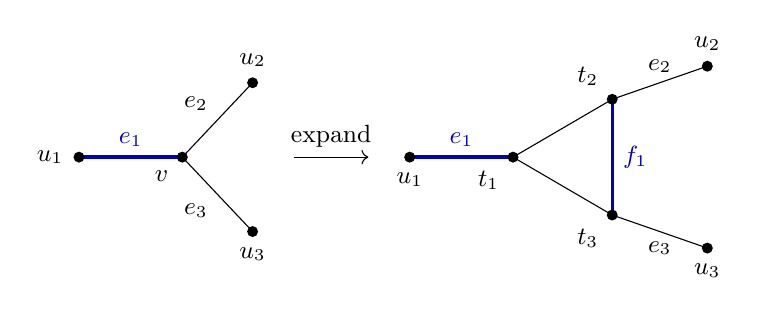
\begin{tikzpicture}[
  x=1.05cm,y=1.05cm,
  matched/.style={very thick,blue!75!black},
  vertex/.style={circle,fill,inner sep=1.4pt},
  every node/.style={font=\small}
]
  \coordinate (v) at (0,0);
  \coordinate (u1) at (-1.25,0);
  \coordinate (u2) at (0.85,0.9);
  \coordinate (u3) at (0.85,-0.9);
  \draw[matched] (u1)--node[above] {\(e_1\)} (v);
  \draw (u2)--node[above left] {\(e_2\)} (v);
  \draw (u3)--node[below left] {\(e_3\)} (v);
  \node[vertex,label=below left:\(v\)] at (v) {};
  \node[vertex,label=left:\(u_1\)] at (u1) {};
  \node[vertex,label=above:\(u_2\)] at (u2) {};
  \node[vertex,label=below:\(u_3\)] at (u3) {};

  \draw[->] (1.35,0)--node[above] {expand} (2.25,0);

  \coordinate (t1) at (4,0);
  \coordinate (t2) at (5.2,0.7);
  \coordinate (t3) at (5.2,-0.7);
  \coordinate (w1) at (2.75,0);
  \coordinate (w2) at (6.35,1.1);
  \coordinate (w3) at (6.35,-1.1);
  \draw[matched] (w1)--node[above] {\(e_1\)} (t1);
  \draw (w2)--node[above] {\(e_2\)} (t2);
  \draw (w3)--node[below] {\(e_3\)} (t3);
  \draw (t1)--(t2) (t1)--(t3);
  \draw[matched] (t2)--node[right] {\(f_1\)} (t3);
  \node[vertex,label=below left:\(t_1\)] at (t1) {};
  \node[vertex,label=above left:\(t_2\)] at (t2) {};
  \node[vertex,label=below left:\(t_3\)] at (t3) {};
  \node[vertex,label=below:\(u_1\)] at (w1) {};
  \node[vertex,label=above:\(u_2\)] at (w2) {};
  \node[vertex,label=below:\(u_3\)] at (w3) {};
\end{tikzpicture}
\caption{A local triangle expansion. The displayed matching uses
\(e_1\); its unique extension crossing the triangle cut once
adds the opposite edge \(f_1\). Thick blue edges are selected.
The rest of the graph is unchanged.}
\label{ex:fig-triangle-expansion}
\end{figure}


\begin{samepage}
\begin{lemma}[The face of a triangle expansion]
\label{ex:lem-expansion-face}
The set
\[
 Q_T=\{y\in P(G'):y(\delta(T))=1\}
\]
is a face of \(P(G')\) affinely isomorphic to \(P(G)\). Under this
isomorphism an old edge keeps its coordinate and
\[
 y_{f_i}=y_{e_i}\qquad(1\le i\le3).
\]
If \(x\in P(G)\) has coordinate \(1/3\) on every edge, its image
\(x'\) has coordinate \(1/3\) on every edge of \(G'\).
The isomorphism maps the minimal face at \(x\) onto the minimal
face at \(x'\).
\end{lemma}
\end{samepage}

\begin{proof}
Every perfect matching of \(G'\) crosses the odd cut
\(\delta(T)\) either once or three times. Hence
\(y(\delta(T))\ge1\) is valid on \(P(G')\), and its equality set
is a face. A convex combination lies in this face exactly when
every matching with positive coefficient crosses the cut once.
For these matchings the extension and contraction just described
are inverse bijections, and the indicator of \(f_i\) equals the
indicator of \(e_i\). They therefore induce the stated affine
isomorphism, with inverse given by restriction to the old edge
labels.

The coordinate statement follows directly. Finally, \(Q_T\) is
a face containing \(x'\). The minimal face of \(P(G')\) at
\(x'\) is therefore also the minimal face of \(Q_T\) at \(x'\);
affine isomorphisms preserve minimal faces.
\end{proof}

\subsection{A triangular minimal face for every order}

Begin with two vertices joined by three distinct labelled parallel
edges. Its three one-edge perfect matchings partition its edge set.
Repeatedly expand any vertex as above. Each expansion adds two
vertices and three edges, and all degrees remain three. Denote
any graph obtained after \(m-1\) expansions by \(G_m\), so that
\[
 |V(G_m)|=2m,\qquad |E(G_m)|=3m.
\]
The three initial perfect matchings extend uniquely at each step.
Their extensions \(M_1,M_2,M_3\) still partition the edge set:
the old edges retain their partition, and \(f_i\) belongs to the
extension of the matching containing \(e_i\). In particular,
\[
 x^{(m)}=\tfrac13\bigl(a(M_1)+a(M_2)+a(M_3)\bigr)
\]
has every coordinate equal to \(1/3\) and belongs to the full
perfect-matching polytope.

The first expansion gives \(K_4\); subsequent expansions preserve
simplicity. Thus \(G_m\) is simple for every \(m\ge2\), and these
are Klee graphs. Only the starting case \(m=1\) needs parallel
edges.

\begin{proposition}[Sharp codimension and prescribed-marginal entropy]
\label{ex:prop-klee-face}
For every integer \(m\ge1\), the graph \(G_m\) and the point
\(x^{(m)}\) above satisfy
\[
 F_{x^{(m)}}=
 \operatorname{conv}\{a(M_1),a(M_2),a(M_3)\},
 \qquad d(x^{(m)})=2.
\]
The unique law on perfect matchings with mean \(x^{(m)}\) is the
uniform law on \(M_1,M_2,M_3\). Consequently,
\begin{equation}
\label{ex:eq-klee-values}
 \begin{aligned}
 |E(G_m)|-d(x^{(m)})&=3m-2,\\
 H(x^{(m)})&=\ln3,\\
 F(x^{(m)})&=m\ln3,\\
 B(x^{(m)})&=2m\ln(3/2).
 \end{aligned}
\end{equation}
\end{proposition}

\begin{proof}
For \(m=1\), the three matching vectors are the three coordinate
vectors in \(\mathbb R^3\), and \(P(G_1)\) is their simplex.
Its uniform point is in its relative interior. Repeated application
of Lemma~\ref{ex:lem-expansion-face} shows that the minimal face at
\(x^{(m)}\) is the image of this simplex, with vertices
\(a(M_1),a(M_2),a(M_3)\). In particular its dimension is two.

One can also see the restriction on laws directly. For the last
inserted triangle, a law with edge marginals \(1/3\) has expected
cut-crossing count \(3(1/3)=1\). Since each matching crosses this
cut once or three times, it must cross once almost surely.
Contraction gives a law on the preceding graph with the same
uniform marginals, and the crossing-one extension is unique.
Iterating leaves only the three initial matchings. Thus the
original law is supported on \(M_1,M_2,M_3\). Since these
matchings partition the edges, the marginal of any edge in
\(M_i\) equals the probability assigned to \(M_i\), which must
be \(1/3\). This proves uniqueness and the entropy formula.

There are \(3m\) edges, all with marginal \(1/3\). Substitution
in the definitions of \(F\) and \(B\) gives the remaining
formulas.
\end{proof}

All coordinates here are strictly between zero and one.
Equation~\eqref{ex:eq-klee-values} therefore attains the bound in
Proposition~\ref{geom:prop-rank} for every \(m\ge1\). Equivalently,
by Equation~\eqref{geom:eq-rank}, the tight odd-cut rows have rank
\(3m-2\). The dimension two is the dimension of the minimal face
at \(x^{(m)}\); the whole perfect-matching polytope can have
additional vertices.

\begin{corollary}[Restriction on a universal entropy coefficient]
\label{ex:cor-coefficient}
If a constant \(c\) satisfies
\[
 H(x)\ge F(x)-cB(x)
\]
for every finite loopless multigraph \(G\) and every
\(x\in P(G)\), then
\[
 c\ge\frac{\ln3}{2\ln(3/2)}.
\]
The same necessary bound holds if the assertion is restricted to
simple graphs.
\end{corollary}

\begin{proof}
Applying the asserted inequality to \(G_m,x^{(m)}\) gives
\[
 c\ge
 \frac{(m-1)\ln3}{2m\ln(3/2)}.
\]
Let \(m\) tend to infinity. The graphs with \(m\ge2\) are simple,
so the same limit applies under that restriction.
\end{proof}

The necessary coefficient in Corollary~\ref{ex:cor-coefficient} lies
strictly between $1$ and the universal coefficient $2$ supplied by
Theorem~\ref{ent:main}. Sharpness of the geometric estimate therefore
does not settle the optimal entropy coefficient. The next example makes
the failure of coefficient one explicit at a fixed order.

\subsection{An eight-vertex obstruction to coefficient one}

For a concrete instance, take vertex set \(\{0,1,\ldots,7\}\) and
edge set
\[
 E=\{01,03,05,14,16,23,24,27,34,56,57,67\},
\]
where \(ij\) denotes the undirected edge with endpoints \(i,j\).
Contracting the triangles \(T=\{2,3,4\}\) and
\(U=\{5,6,7\}\) gives \(K_4\). Thus this graph is obtained by
expanding two vertices of \(K_4\), and is an instance of \(G_4\).

Its five perfect matchings are
\[
 \begin{aligned}
 M_1&=\{01,27,34,56\},&
 M_2&=\{03,16,24,57\},\\
 M_3&=\{05,14,23,67\},&
 N_1&=\{03,14,27,56\},\\
 &&N_2&=\{05,16,27,34\}.
 \end{aligned}
\]
This list follows without enumeration software. A matching uses
one of \(01,03,05\). If it uses \(01\), the remaining two odd
triangles are joined only by \(27\), forcing \(M_1\). If it uses
\(03\), vertex \(1\) is matched by \(14\) or \(16\), after which
the remaining edges are forced, giving \(N_1\) or \(M_2\).
If it uses \(05\), the same two choices at vertex \(1\) force
\(M_3\) or \(N_2\).

The cuts
\[
 \delta(T)=\{03,14,27\},\qquad
 \delta(U)=\{05,16,27\}
\]
both have total marginal one at \(x_e=1/3\).
The matching \(N_1\) crosses the first cut three times, and
\(N_2\) crosses the second cut three times. They therefore have
probability zero in every law with those marginals. The remaining
three matchings partition \(E\), so their probabilities are all
\(1/3\). In particular the relevant entropy is \(\ln3\), even
though the graph has five perfect matchings in total.

At this feasible point of the full polytope,
\[
 H(x)=\ln3,\qquad
 F(x)-B(x)=4\ln(4/3)>\ln3,
\]
because \( (4/3)^4=256/81>3\).
The difference \(F(x)-B(x)-H(x)\) is
\(\ln(256/243)>0\). This gives a simple eight-vertex
counterexample to the coefficient-one lower bound.

\section{Weighted partition functions}\label{cons:weighted-section}
\label{d:sec-weighted-interface}

Let $G$ be a loopless labelled multigraph on $n=2m\ge2$ vertices with
at least one perfect matching. Write $P=P(G)$. We pass from natural-log
entropy to binary-log weights, so that the resulting estimate can be
used by the rational counting algorithm.

Put
\[
 h_2(x)=\frac{F(x)}{\ln2}=\sum_{e\in E}-x_e\log_2x_e,
 \qquad 0\log_2 0=0.
\]
For \(\beta\in\mathbb R^E\), define
\begin{equation}
 \label{cons:weighted-definitions}
 Z_\beta=\sum_{M\in\mathcal M(G)}2^{\beta\cdot\mathbf1_M},
 \qquad
 q^*=\max_{x\in P}
        [h_2(x)+\beta\cdot x].
\end{equation}
The maximum exists by continuity on the compact matching polytope.

\begin{corollary}[Weighted counting estimate]
\label{cons:weighted}
For every finite real vector \(\beta\),
\begin{equation}
 \label{cons:weighted-bracket}
                q^*-\frac{2m-2}{\ln2}
                \le\log_2 Z_\beta\le q^*.
\end{equation}
\end{corollary}

\begin{proof}
Let \(p_\beta(M)=2^{\beta\cdot\mathbf1_M}/Z_\beta\), a positive
probability law on the matching family. The finite entropy comparison
with this law gives, for any matching law \(p\) of mean \(x\),
\[
 \frac{-\sum_Mp(M)\ln p(M)}{\ln2}+\beta\cdot x
                          \le\log_2 Z_\beta,
\]
with equality for \(p=p_\beta\). Indeed, this is the nonnegativity
of \(\sum_{M:p(M)>0}p(M)\ln(p(M)/p_\beta(M))\), which follows
from \(\ln t\le t-1\).
Taking a maximizing law at each mean and then the maximum over means
therefore yields
\begin{equation}
 \label{cons:variational}
 \log_2 Z_\beta
       =\max_{x\in P}\left[\frac{H(x)}{\ln2}+\beta\cdot x\right].
\end{equation}
Corollary~\ref{cons:defect} says
\(F(x)-(2m-2)\le H(x)\le F(x)\).
Divide by \(\ln2\), add \(\beta\cdot x\), and maximize to obtain
Equation~\eqref{cons:weighted-bracket}.
\end{proof}

The analytical comparison does not itself supply a numerical optimizer.
The exact-arithmetic construction in
Sections~\ref{d:sec-objective}--\ref{d:sec-algorithm} uses the following
coarser bracket, with fixed constants that leave room for its later
rounding and optimization errors.

\begin{corollary}[Conservative weighted bracket]
\label{d:coarse-weighted}
For every finite loopless labelled multigraph on an even number
\(n\ge2\) of vertices with at least one perfect matching, and every
finite real vector \(\beta\in\mathbb R^E\),
\begin{equation}
 \label{d:eq-coarse-weighted}
 q^*-4n\le\log_2 Z_\beta\le q^*+n.
\end{equation}
\end{corollary}

\begin{proof}
With \(n=2m\), Corollary~\ref{cons:weighted} gives
\[
 q^*-\frac{n-2}{\ln2}\le\log_2Z_\beta\le q^*.
\]
Since \(\ln2=\int_1^2t^{-1}\,dt\ge1/2\), we have
\((n-2)/\ln2\le2n-4\le4n\). Enlarging both sides of this bracket
proves the claim.
\end{proof}

For the empty graph, the matching family consists of the
empty matching, \(Z_\beta=1\) and \(q^*=0\). The counting algorithm
handles that input directly. On positive even order it uses exactly
Equation~\eqref{d:eq-coarse-weighted}; all constants in the finite
optimization and final estimate below refer to this bracket.

\section{A rational objective for counting matchings}
\label{d:sec-objective}

The weighted entropy estimate reduces counting to a continuous maximum.
We now replace that maximum by one computed from exact rational data.
Assume throughout this section that \(n\ge4\) is even.  Let \(N\) be the
number of perfect matchings in the input graph, with parallel edges
counted as distinct choices.  We allow the multiplicity \(k_e\) of each
unordered pair \(e\in\binom V2\) to be supplied in binary; an absent pair
has \(k_e=0\).  For a simple graph, every multiplicity is zero or one.

We work on the complete simple graph \(K_n\), writing
\[
  P=P(K_n),\qquad p=\binom n2.
\]
The objective functions below have one coordinate for each of these
\(p\) unordered pairs.  In particular, \(P\) is nonempty even when
the input graph has no perfect matching. Small positive weights on absent
pairs will encode the input support in the objective. Completion also
provides the uniform feasible mean \(u_{ij}=1/(n-1)\), whose nontrivial
odd-cut inequalities are strict. Section~\ref{d:sec-optimization} uses
that slack to repair cut violations after correcting the degree sums.

\subsection{Completing the graph with small weights}

Set
\begin{equation}
\label{d:eq-completion-weights}
\begin{split}
 b_{\max}&=\max\bigl(\{0\}\cup
       \{\lfloor\log_2 k_e\rfloor:k_e>0\}\bigr),\\
 L&=100(n+b_{\max}+1)^3,\qquad
 \beta_e=
 \begin{cases}
   \lfloor\log_2 k_e\rfloor,&k_e>0,\\
   -L,&k_e=0.
 \end{cases}
\end{split}
\end{equation}
For a positive integer \(k_e\), its binary bit length minus one equals
\(\lfloor\log_2 k_e\rfloor\).  Thus these coefficients are computed
exactly by integer arithmetic, and their numerical magnitudes are
polynomial in \(n+b_{\max}\).

Use \(Z_\beta\) and \(q^*\) from Corollary~\ref{d:coarse-weighted} for \(K_n\)
with the weights in Equation~\eqref{d:eq-completion-weights}.  A term in
\(Z_\beta\) is called valid if its matching uses only pairs with positive
input multiplicity; write \(Z_{\mathrm{good}}\) and
\(Z_{\mathrm{bad}}\) for the sums of valid and remaining terms,
respectively.

\begin{lemma}[Weighted completion]
\label{d:lem-penalized-count}
The contribution of matchings using an absent pair satisfies
\[
  0\le Z_{\mathrm{bad}}\le2^{-20n}.
\]
Moreover,
\begin{equation}
\label{d:eq-penalized-count}
\begin{aligned}
 N=0&\quad\Longrightarrow\quad \log_2 Z_\beta\le-20n,\\
 N>0&\quad\Longrightarrow\quad
       \max\{1,2^{-n/2}N\}\le Z_\beta\le2N.
\end{aligned}
\end{equation}
\end{lemma}

\begin{proof}
For each pair with \(k_e>0\), put
\(r_e=2^{\lfloor\log_2 k_e\rfloor}\).  Then
\[
  \frac{k_e}{2}\le r_e\le k_e.
\]
For a valid matching of \(K_n\), the product of its \(k_e\)'s is the
number of corresponding perfect matchings in the input multigraph.
Replacing these \(n/2\) factors by \(r_e\) and summing therefore gives
\begin{equation}
\label{d:eq-valid-rounded-count}
  2^{-n/2}N\le Z_{\mathrm{good}}\le N.
\end{equation}
If \(N>0\), there is at least one valid matching, and its rounded
weight is a positive integer.  Hence \(Z_{\mathrm{good}}\ge1\).

Every remaining matching uses a pair of weight \(2^{-L}\), and each
of its other pair weights is at most \(2^{b_{\max}}\).  There are at most
\(2^p\) matchings, since each is a subset of the \(p\) pairs.  Thus
\[
  Z_{\mathrm{bad}}\le 2^{p+b_{\max}n/2-L}\le2^{-20n}.
\]
For the last inequality, put \(t=n+b_{\max}+1\ge5\) and note that
\[
  p+\frac{b_{\max}n}{2}+20n\le t^2+20t\le100t^3=L.
\]
When \(N=0\), every term is in \(Z_{\mathrm{bad}}\); also \(Z_\beta>0\)
because \(K_n\) has a perfect matching and every assigned weight is
positive.  This proves the first implication in
Equation~\eqref{d:eq-penalized-count}.
When \(N>0\), Equation~\eqref{d:eq-valid-rounded-count} gives the lower
bounds, while
\[
  Z_\beta\le N+2^{-20n}\le2N
\]
because \(N\) is a positive integer.
\end{proof}

\subsection{Interpolating entropy on a dyadic grid}

Let \(K\) be the least nonnegative integer such that \(2^K\ge p\).
Define \(\phi(t)=-t\log_2 t\) on \([0,1]\), with \(\phi(0)=0\), and
let \(\psi\) be its continuous linear interpolant at
\[
  0,\ 2^{-K},\ 2^{-(K-1)},\ \ldots,\ 2^{-1},\ 1.
\]
The interpolant has the explicit rational formulas
\begin{equation}
\label{d:eq-dyadic-chords}
 \psi(t)=
 \begin{cases}
   Kt,&0\le t\le2^{-K},\\
   (k-1)t+2^{-k},
     &2^{-(k+1)}\le t\le2^{-k},\quad 0\le k<K.
 \end{cases}
\end{equation}
The formulas agree at common endpoints.

\begin{lemma}[Dyadic entropy approximation]
\label{d:lem-dyadic-entropy}
The function \(\psi\) is concave, with integer slopes of absolute value
at most \(K\).  For every \(x\in P\),
\begin{equation}
\label{d:eq-dyadic-entropy-error}
  0\le h_2(x)-\sum_e\psi(x_e)
     \le\frac n2+1\le n.
\end{equation}
\end{lemma}

\begin{proof}
At a positive knot, \(\phi(2^{-k})=k2^{-k}\).  The chord between
\(2^{-(k+1)}\) and \(2^{-k}\) therefore has slope \(k-1\) and
intercept \(2^{-k}\), whereas the chord from zero has slope \(K\).
This proves Equation~\eqref{d:eq-dyadic-chords}.  Reading the intervals
from left to right, the slopes are nonincreasing, so \(\psi\) is
concave.  Since \(p\ge6\), we have \(K\ge1\), and all its slopes lie
between \(-1\) and \(K\).

The concavity of \(\phi\) puts every chord below its graph.  If
\(2^{-(k+1)}\le t\le2^{-k}\), then
\[
  \psi(t)-kt=2^{-k}-t\ge0,
  \qquad \phi(t)\le(k+1)t.
\]
Consequently \(0\le\phi(t)-\psi(t)\le t\) on this interval.
On the interval adjacent to zero, write \(t=2^{-K}r\), where
\(0\le r\le1\).  Then
\[
  \phi(t)-\psi(t)=2^{-K}(-r\log_2 r)\le2^{-K}.
\]
Here the expression at \(r=0\) is interpreted by continuity; on
\((0,1]\), differentiation gives the maximum
\(1/(e\ln2)<1\).

For \(x\in P\), summing the degree equations gives
\(\sum_e x_e=n/2\).  Apply the bound \(x_e\) on intervals above
\(2^{-K}\), and the bound \(2^{-K}\) on the interval below it.
The total error is at most
\[
  \sum_{e:x_e\ge2^{-K}}x_e
     +\bigl|\{e:x_e<2^{-K}\}\bigr|\,2^{-K}
  \le \frac n2+p2^{-K}
  \le \frac n2+1
  \le n.
\]
This proves Equation~\eqref{d:eq-dyadic-entropy-error}.
\end{proof}

Define the concave function \(f\) on the entire box \([0,1]^p\) by
\begin{equation}
\label{d:eq-surrogate-objective}
  f(x)=\sum_e\psi(x_e)+\beta\cdot x,\qquad
  f^*=\max_{x\in P}f(x).
\end{equation}
Equation~\eqref{d:eq-dyadic-entropy-error} gives
\(f(x)\le h_2(x)+\beta\cdot x\le f(x)+n\) on \(P\).
Taking maxima yields
\begin{equation}
\label{d:eq-surrogate-gap}
  f^*\le q^*\le f^*+n.
\end{equation}
On each affine piece, \(f\) has integer coordinate slopes of absolute
value at most \(K+L\), since \(|\beta_e|\le L\).  All breakpoints and
intercepts in Equation~\eqref{d:eq-dyadic-chords} have denominators
dividing \(2^K<2p\).  Thus \(f\) can be evaluated exactly at rational
points using rational arithmetic.  Section~\ref{d:sec-optimization}
uses these properties to estimate \(f^*\).

\section{Optimization by an exact penalty}
\label{d:sec-optimization}

Retain the notation of Section~\ref{d:sec-objective}: \(n\ge4\) is even,
\(P=P(K_n)\), \(p=\binom n2\), and
\(f^*=\max_{x\in P}f(x)\).
We first replace optimization over \(P\) by optimization over the box
\([0,1]^p\).  For \(x\) in this box, define
\begin{equation}
\label{d:eq-max-violation}
w(x)=
\max\left\{
0,\ 
\max_{i\in V}\bigl|x(\delta(i))-1\bigr|,\ 
\max_{\substack{S\subseteq V\\ |S|\ \text{odd}}}
       \bigl(1-x(\delta(S))\bigr)
\right\}.
\end{equation}
By Theorem~\ref{geom:thm-polytope}, \(w(x)=0\) exactly when \(x\in P\).

\begin{lemma}[Feasibility repair]
\label{d:lem-feasibility-repair}
Set \(A_0=10n^2\).  For every \(x\in[0,1]^p\), there is \(y\in P\) such that
\[
\|y-x\|_\infty\le (2+A_0)w(x).
\]
\end{lemma}

\begin{proof}
Write \(w=w(x)\), \(d_i=1-x(\delta(i))\), and
\(d_{\mathrm{tot}}=\sum_{i\in V}d_i\).  Correct the degrees by setting
\begin{equation}
\label{d:eq-degree-correction}
x'_{ij}
=x_{ij}+\frac{d_i+d_j}{n-2}
          -\frac{d_{\mathrm{tot}}}{(n-2)(n-1)}
\qquad (i\ne j).
\end{equation}
The correction sums to \(d_i\) at vertex \(i\), since
\[
\sum_{j\ne i}(d_i+d_j)=(n-2)d_i+d_{\mathrm{tot}}.
\]
Thus \(x'(\delta(i))=1\) for every \(i\).  Since
\(|d_i|\le w\) and \(|d_{\mathrm{tot}}|\le nw\),
\[
\|x'-x\|_\infty
\le
\left(\frac{2}{n-2}+\frac{n}{(n-2)(n-1)}\right)w
\le 2w.
\]
Consequently \(x'_e\ge-2w\), and every odd set \(S\) satisfies
\begin{equation}
\label{d:eq-corrected-cut-bound}
x'(\delta(S))\ge 1-(1+2p)w.
\end{equation}

Let \(u_{ij}=1/(n-1)\).  This vector has degree sums one, and
\[
u(\delta(S))=\frac{|S|(n-|S|)}{n-1}.
\]
Cuts with \(|S|=1\) or \(|S|=n-1\) have value one.  For every nontrivial
odd cut, \(3\le |S|\le n-3\), and hence, when \(n\ge6\),
\[
u(\delta(S))\ge\frac{3(n-3)}{n-1}\ge\frac32.
\]
There are no nontrivial odd cuts when \(n=4\).  In particular, \(u\in P\).

Set
\begin{equation}
\label{d:eq-uniform-repair}
t=\min\{1,A_0w\},
\qquad
y=(1-t)x'+tu.
\end{equation}
If \(A_0w\ge1\), including equality, then \(y=u\in P\).
Otherwise \(t=A_0w<1\).  The inequalities
\[
\frac{A_0}{n-1}\ge2,
\qquad
\frac{A_0}{2}\ge1+2p
\]
give
\[
y_e\ge-2(1-t)w+\frac{A_0w}{n-1}\ge0.
\]
Equation~\eqref{d:eq-corrected-cut-bound} also gives, for each nontrivial
odd cut,
\[
y(\delta(S))
\ge 1-(1-t)(1+2p)w+\frac{A_0w}{2}
\ge1.
\]
The degree sums remain one, so the trivial odd cuts also have value one.
Theorem~\ref{geom:thm-polytope} now yields \(y\in P\) in this branch
as well.

For either branch, use the identity
\[
y-x=(1-t)(x'-x)+t(u-x).
\]
Both \(u\) and \(x\) lie in the box, so
\[
\|y-x\|_\infty
\le 2(1-t)w+t\|u-x\|_\infty
\le 2w+t
\le (2+A_0)w.
\]
This also covers \(w=0\).
\end{proof}

The repair bound converts constraint violation into a quantitative distance
from feasibility. We can therefore penalize violations by a fixed amount
large enough to recover exactly the constrained optimum.

Define the positive integers \(M_0,D_0\) and the function \(\Phi\) by
\begin{equation}
\label{d:eq-penalty-parameters}
M_0=p(K+L)(2+A_0),\qquad
\Phi(x)=f(x)-M_0w(x),\qquad
D_0=p(K+L+M_0)^2.
\end{equation}
A vector \(g\) is a \emph{supergradient} of \(\Phi\) at \(x\) on the box if
\[
\Phi(z)\le \Phi(x)+g\cdot(z-x)
\qquad\text{for every }z\in[0,1]^p.
\]

\begin{lemma}[Exact penalty and integral supergradients]
\label{d:lem-exact-penalty}
The function \(\Phi\) is concave on \([0,1]^p\), and
\[
\max_{x\in[0,1]^p}\Phi(x)=f^*.
\]
At every point of the box, \(\Phi\) has an integral supergradient \(g\)
satisfying \(\|g\|_2^2\le D_0\).
\end{lemma}

\begin{proof}
By Lemma~\ref{d:lem-dyadic-entropy}, the slopes of \(\psi\) are integers of
absolute value at most \(K\).  Since \(|\beta_e|\le L\), it follows that
\begin{equation}
\label{d:eq-objective-lipschitz}
|f(x)-f(y)|\le (K+L)\sum_e|x_e-y_e|
            \le p(K+L)\|x-y\|_\infty
\qquad (x,y\in[0,1]^p).
\end{equation}
For the point \(y\in P\) supplied by Lemma~\ref{d:lem-feasibility-repair},
Equation~\eqref{d:eq-objective-lipschitz} gives
\[
\Phi(x)
\le f(y)+p(K+L)\|x-y\|_\infty-M_0w(x)
\le f(y)\le f^*.
\]
Conversely, \(\Phi=f\) on \(P\), proving equality of the maxima.
The function \(w\) is a maximum of affine functions and is therefore
convex.  Since \(f\) is concave, \(\Phi\) is concave.

Choose a supporting piece slope \(\sigma_e\) of \(\psi\) at each \(x_e\);
at a knot either adjacent slope is allowed.  With
\(b_e=\sigma_e+\beta_e\), these choices give
\[
f(z)\le f(x)+b\cdot(z-x)
\qquad (z\in[0,1]^p).
\]
Write each absolute value in Equation~\eqref{d:eq-max-violation} as the
maximum of its two affine terms.  Choose any active affine term
\(a\cdot z+c\) in this maximum, including the zero term when it is active.
Then \(a_e\in\{-1,0,1\}\), and
\[
w(z)\ge a\cdot z+c=w(x)+a\cdot(z-x).
\]
Subtracting the last inequality, multiplied by \(M_0\), proves that
\(g=b-M_0a\) is a supergradient of \(\Phi\) on the entire box.
The independent choices of supporting pieces and active rows are valid
also at endpoints and ties.  Finally, \(g\) is integral and
\[
|g_e|\le K+L+M_0,
\qquad
\|g\|_2^2\le p(K+L+M_0)^2=D_0.
\]
\end{proof}

We use the classical projected subgradient method
\citep[Equation~(1)]{Polyak1967} to approximate the maximum of \(\Phi\).
Its bounded integral supergradients permit a fixed step size and keep
every iterate on one rational grid. The next lemma gives the finite
iteration count and value guarantee directly.

\begin{lemma}[Finite projected ascent]
\label{d:lem-projected-ascent}
Let \(N_{\mathrm{it}}=pD_0\), set \(x^{(0)}=0\), and for
\(j=0,\ldots,N_{\mathrm{it}}-1\) choose a supergradient
\(g^{(j)}\) as in Lemma~\ref{d:lem-exact-penalty} and set
\begin{equation}
\label{d:eq-projected-iterations}
x^{(j+1)}
=\Pi_{[0,1]^p}\left(x^{(j)}+\frac{g^{(j)}}{D_0}\right),
\end{equation}
where \(\Pi_{[0,1]^p}\) clips each coordinate to \([0,1]\).
Then
\begin{equation}
\label{d:eq-optimization-accuracy}
R=\left\lfloor\max_{0\le j<N_{\mathrm{it}}}\Phi(x^{(j)})\right\rfloor
\qquad\text{satisfies}\qquad
R\le f^*\le R+2.
\end{equation}
\end{lemma}

\begin{proof}
Choose \(z\in P\) with \(f(z)=f^*\); then \(\Phi(z)=f^*\) by
Lemma~\ref{d:lem-exact-penalty}.  Clipping cannot increase distance to
\(z\in[0,1]^p\).  Expanding the squared distance and using the
supergradient inequality therefore gives
\begin{align}
\|x^{(j+1)}-z\|_2^2
&\le \|x^{(j)}-z\|_2^2
 +\frac{2}{D_0}g^{(j)}\cdot(x^{(j)}-z)
 +\frac{\|g^{(j)}\|_2^2}{D_0^2}\notag\\
&\le \|x^{(j)}-z\|_2^2
 -\frac{2}{D_0}\bigl(f^*-\Phi(x^{(j)})\bigr)+\frac1{D_0}.
\label{d:eq-ascent-step}
\end{align}
Summing Equation~\eqref{d:eq-ascent-step} over exactly the indicated
\(N_{\mathrm{it}}\) indices yields
\begin{align*}
2\sum_{j=0}^{N_{\mathrm{it}}-1}
  \bigl(f^*-\Phi(x^{(j)})\bigr)
&\le D_0\bigl(\|x^{(0)}-z\|_2^2
             -\|x^{(N_{\mathrm{it}})}-z\|_2^2\bigr)
       +N_{\mathrm{it}}\\
&\le pD_0+N_{\mathrm{it}}=2N_{\mathrm{it}}.
\end{align*}
Here \(\|x^{(0)}-z\|_2^2\le p\).
Thus the largest of the sampled values, say \(V\), satisfies
\(f^*-1\le V\le f^*\).  Since \(R=\lfloor V\rfloor\),
\[
R\le V\le f^*,
\qquad
f^*\le V+1<R+2,
\]
which proves Equation~\eqref{d:eq-optimization-accuracy}.
\end{proof}

Every iterate in Equation~\eqref{d:eq-projected-iterations} has coordinates
that are integer multiples of \(1/D_0\): the update adds an integral
vector divided by \(D_0\), and clipping inserts only \(0\) or \(1\).
To evaluate \(w\) and choose an active row, compare the zero term and the
\(2n\) signed degree terms with the largest odd-cut violation.
Lemma~\ref{d:lem-odd-cut-oracle} computes a minimum odd cut from the
nonnegative integer capacities \(D_0x_e^{(j)}\) and returns its row in the
original edge coordinates.  The values of \(\Phi\) and the floor defining
\(R\) can then be computed exactly using rational arithmetic.
Proposition~\ref{d:prop-bit-complexity} gives the resulting bit-complexity
bound.

\section{Computing an active odd-cut constraint}
\label{d:sec-odd-cuts}

The optimization in Section~\ref{d:sec-optimization} needs both the value of
\(w(x)\) and an affine function attaining its defining maximum.
The degree violations are immediate to compute.  We supply the remaining
ingredient: an exact minimum odd cut, together with its vertex set.
The use of minimum odd cuts for matching-constraint separation goes back
to Padberg and Rao~\citep{PadbergRao1982}. We prove the recursion and its
arithmetic bounds here.

Throughout this section, an auxiliary graph has vertex set \(W\) and
nonnegative integer capacities \(c_{ij}=c_{ji}\) for distinct \(i,j\in W\).
Absent edges have capacity zero.  Parallel capacities are summed and loops
are discarded.  Write
\[
 c(S)=\sum_{\substack{i\in S\\ j\in W\setminus S}}c_{ij},
 \qquad
 C=\sum_{\{i,j\}\subseteq W}c_{ij},
 \qquad v=|W|.
\]

We use the classical augmenting-path method of Ford and Fulkerson
\citep[Section~2]{FordFulkerson1957}, specialized here to unit
augmentations. The capacity-dependent bound needed below is proved
explicitly.

\begin{lemma}[An integral two-terminal minimum cut]
\label{d:lem-unit-mincut}
For distinct \(a,b\in W\), a minimum cut separating \(a\) from \(b\)
can be found deterministically using at most \(C\) unit augmentations
and \(O(v^2(C+1))\) arithmetic operations on integers of
\(O(\log_2(v+C+2))\) bits.
\end{lemma}

\begin{proof}
Maintain integers \(b_{ij}=-b_{ji}\) such that
\(b_{ij}\le c_{ij}\) in both directions and
\(\sum_j b_{ij}=0\) for \(i\notin\{a,b\}\).
The two directional inequalities give
\(-c_{ij}\le b_{ij}\le c_{ij}\).
Start with zero flow.  If a simple directed path from \(a\) to \(b\)
uses only steps with residual capacity \(c_{ij}-b_{ij}>0\), increase
the flow on each forward step by one and decrease its reverse by one.
Integrality makes this feasible, conservation is preserved, and the
net source outflow \(q=\sum_j b_{aj}\) increases by one.
Since
\[
 q\le \sum_j c_{aj}\le C,
\]
there are at most \(C\) augmentations.

When no such path exists, let \(S\) be the vertices reachable from \(a\)
by positive-residual steps.  Then \(b\notin S\), and every step from
\(S\) to its complement is saturated.  Antisymmetry cancels internal
flows, so conservation gives
\[
 q=\sum_{\substack{i\in S\\j\notin S}}b_{ij}
   =\sum_{\substack{i\in S\\j\notin S}}c_{ij}=c(S).
\]
For every other \(a\)--\(b\) cut, the same conservation identity and
\(b_{ij}\le c_{ij}\) give capacity at least \(q\).  Thus \(S\) is minimum.
A graph search with fixed vertex order finds a simple residual path,
or the final reachable set, in \(O(v^2)\) operations.  There are at most
\(C+1\) searches, and all flows and residual capacities have magnitude
at most \(2C\).  The argument includes \(C=0\).
\end{proof}

\begin{lemma}[Minimum odd-terminal cut]
\label{d:lem-odd-cut-oracle}
Let \(U\subseteq W\) have positive even cardinality.  One can
deterministically find a set \(S\subseteq W\) minimizing \(c(S)\)
subject to \(|S\cap U|\) being odd.  The algorithm returns the set itself,
uses at most \(|U|-1\) recursive instances, and requires
\(O(|U|^3v^2(C+1))\) arithmetic operations on integers of
\(O(\log_2(v+C+2))\) bits.
\end{lemma}

\begin{proof}
Call a cut \emph{terminal-separating} if both sides meet \(U\).
Compute a minimum cut for every pair of distinct terminals using
Lemma~\ref{d:lem-unit-mincut}, and take the least-capacity result,
with sides \(A\) and \(\overline A=W\setminus A\).
This is a minimum terminal-separating cut: every such cut separates
some terminal pair, and every recorded pair cut is terminal-separating.

If \(|A\cap U|\) is odd, return \(A\).  Every admissible odd-terminal
cut is terminal-separating, so this answer is optimal.
Otherwise both \(A\cap U\) and \(\overline A\cap U\) have positive even
cardinality.  Form two children:
\begin{enumerate}[label=(\roman*),nosep]
\item keep \(A\), contract \(\overline A\) to a new nonterminal, and
      use terminal set \(A\cap U\);
\item keep \(\overline A\), contract \(A\) to a new nonterminal, and
      use terminal set \(\overline A\cap U\).
\end{enumerate}
For example, in the first child the capacity from \(i\in A\) to the
new vertex is \(\sum_{j\in\overline A}c_{ij}\).
Recurse on both children and return the better lifted cut.
Every call strictly decreases the positive even terminal count;
when \(|U|=2\), the first cut is already odd.

\paragraph{Lifting cuts.}
A child cut lifts by replacing its contracted vertex, if included,
with the entire block it represents.  The crossing capacities are
unchanged, and including that block adds an even number of parent
terminals.  Thus the lift has the same capacity and is terminal-odd.

This remains true through arbitrarily nested contractions.
Relative to the initial instance, current vertices form a partition
into blocks.  Every current terminal is an original terminal singleton,
and every nonterminal block contains an even number of original terminals.
Initially the latter count is zero; each contraction combines an even
number of current terminals with blocks of even parity, preserving
the assertion.  Capacities between current vertices are sums of
original capacities between their blocks.
Consequently every returned subset lifts to an original subset with
the same capacity and terminal parity.
Figure~\ref{d:fig-odd-cut-lift} illustrates the parity rule.

\paragraph{Preserving an optimum.}
Let \(S\) be an optimal odd-terminal side in the current instance.
Exactly one of \(S\cap A\) and \(S\cap\overline A\) contains an odd number
of terminals; exchange the names of the two sides so that it is \(S\cap A\).
Because \(|A\cap U|\) is even, replacing \(S\) by its complement
preserves this odd intersection.  Make this replacement if \(S\)
contains all terminals of \(\overline A\).
Now \(S\cup A\) contains terminals of \(A\) and omits a terminal of
\(\overline A\), so
\[
 c(S\cup A)\ge c(A).
\]
For any two vertex sets, nonnegative undirected capacities satisfy
\begin{equation}
\label{d:eq-cut-submodularity}
 c(S\cap A)+c(S\cup A)\le c(S)+c(A).
\end{equation}
Indeed, the right side minus the left side is twice the capacity
between \(S\setminus A\) and \(A\setminus S\).
It follows that \(c(S\cap A)\le c(S)\).
The set \(S\cap A\) is a feasible odd-terminal side in the first child,
avoiding its contracted vertex.  Hence at least one child has optimum
at most the parent's.  Conversely, lifting shows that every child
optimum is at least the parent's.  Induction on \(|U|\) proves that
the better recursive answer attains the parent optimum.

\paragraph{Size and running time.}
Each nonleaf splits its terminal set into two disjoint nonempty even
sets.  There are at most \(|U|/2\) leaves and hence at most \(|U|-1\)
instances in this binary recursion tree.
Each contracted side contains at least two terminals, so a child
also has fewer vertices than its parent.
Within any one instance, every surviving capacity sums a disjoint
set of original edge capacities; original edges internal to blocks
are discarded.  Its total capacity is therefore at most \(C\).
Capacities in different children may overlap, and we account for them
by multiplying the cost of an instance by the number of instances.

There are at most \(O(|U|^2)\) pair computations per instance,
each costing \(O(v^2(C+1))\) by Lemma~\ref{d:lem-unit-mincut}.
Contractions and lifted-set bookkeeping fit within the same bound.
This proves the stated running time.
All comparisons and tie choices may use fixed orderings; zero
capacities require no perturbation.
\end{proof}

\begin{figure}[tb]
\centering
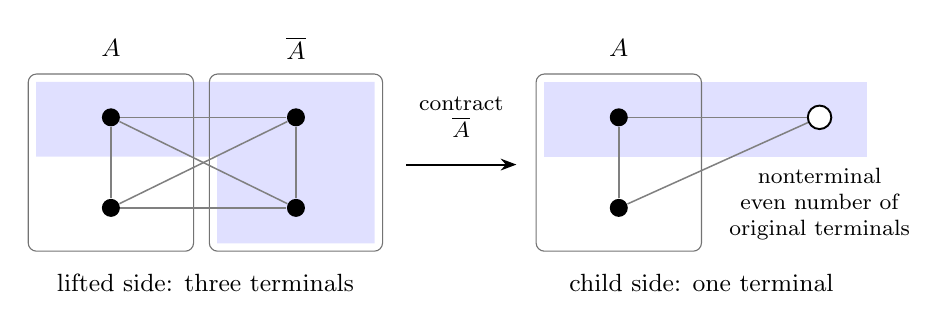
\begin{tikzpicture}[
  x=1cm,y=1cm,
  terminal/.style={circle,fill=black,inner sep=2.3pt},
  contracted/.style={circle,draw=black,fill=white,line width=.7pt,inner sep=3pt},
  block/.style={draw=black!55,rounded corners=3pt},
  cutshade/.style={fill=blue!12,draw=none},
  edge/.style={draw=black!50,line width=.55pt},
  every node/.style={font=\small}
]
\path[cutshade] (0.25,1.3)--(2.55,1.3)--(2.55,.2)--(4.55,.2)
               --(4.55,2.25)--(.25,2.25)--cycle;
\draw[block] (.15,.1) rectangle (2.25,2.35);
\draw[block] (2.45,.1) rectangle (4.65,2.35);
\node at (1.2,2.68) {$A$};
\node at (3.55,2.68) {$\overline A$};
\node[terminal] (a1) at (1.2,1.8) {};
\node[terminal] (a2) at (1.2,.65) {};
\node[terminal] (b1) at (3.55,1.8) {};
\node[terminal] (b2) at (3.55,.65) {};
\draw[edge] (a1)--(a2);
\draw[edge] (a1)--(b1);
\draw[edge] (a1)--(b2);
\draw[edge] (a2)--(b1);
\draw[edge] (a2)--(b2);
\draw[edge] (b1)--(b2);
\node at (2.4,-.3) {lifted side: three terminals};

\draw[-{Stealth[length=2mm]},line width=.7pt]
  (4.95,1.2)--(6.35,1.2);
\node[align=center,font=\footnotesize] at (5.65,1.8)
  {contract\\$\overline A$};

\path[cutshade] (6.7,1.3) rectangle (10.8,2.25);
\draw[block] (6.6,.1) rectangle (8.7,2.35);
\node at (7.65,2.68) {$A$};
\node[terminal] (c1) at (7.65,1.8) {};
\node[terminal] (c2) at (7.65,.65) {};
\node[contracted] (z) at (10.2,1.8) {};
\draw[edge] (c1)--(c2);
\draw[edge] (c1)--(z);
\draw[edge] (c2)--(z);
\node[align=center,font=\footnotesize] at (10.2,.7)
  {nonterminal\\even number of\\original terminals};
\node at (8.7,-.3) {child side: one terminal};
\end{tikzpicture}
\caption{Lifting through an even-terminal contraction.
Filled dots are terminals and the open dot represents the contracted
block.  In this schematic instance each side initially has two terminals.
The shaded child side lifts to the shaded parent side by taking the
entire contracted block, preserving odd parity.  Parallel crossing
capacities are added, so the cut capacity is preserved as well.}
\label{d:fig-odd-cut-lift}
\end{figure}


\paragraph{Recovering an active row in the original coordinates.}
At an optimization trial point, \(D_0x_e\) is a nonnegative integer
for every original complete-graph pair \(e\).
Indeed, the initial point is zero, and an integral supergradient step
of size \(1/D_0\), followed by clipping to \([0,1]\), preserves this grid.
Apply Lemma~\ref{d:lem-odd-cut-oracle} with \(U=V\) and capacities
\(c_e=D_0x_e\).  Store each contracted vertex's block of original
vertices, so the returned cut yields an explicit original set
\(S\subseteq V\) of odd cardinality.  It minimizes \(x(\delta(S))\).

The corresponding affine function in the definition of \(w\) is
\[
 \ell_S(y)=1-\sum_{e\in\delta(S)}y_e.
\]
Its coefficient is \(-1\) on \emph{every} original pair crossing \(S\),
including pairs with \(x_e=0\), and zero elsewhere.
Thus the row is recovered by scanning the original pairs, even if
zero-capacity edges were omitted during graph searches.
Edges discarded as contraction loops have both endpoints in one
block and do not cross a lifted cut.
Comparing \(\ell_S(x)\) with zero and the two signed degree violations
for every vertex gives \(w(x)\) and an affine row attaining it, as
required in Section~\ref{d:sec-optimization}.

Here the initial total capacity is at most \(pD_0\).
A merged edge can exceed \(D_0\), but the bound on each instance's
total capacity remains \(pD_0\); likewise a large reverse residual
does not change the source-outflow bound in Lemma~\ref{d:lem-unit-mincut}.
One complete violation computation therefore takes
\[
 O\!\left(n^5(pD_0+1)\right)
\]
arithmetic operations.
The numerical bounds on \(D_0\) and the resulting bit complexity
are recorded in Proposition~\ref{d:prop-bit-complexity}.

\section{The algorithm and its guarantee}
\label{d:sec-algorithm}

We now assemble the preceding constructions into a deterministic algorithm.
The input consists of a vertex set \(V=\{1,\ldots,n\}\) and nonnegative
integer multiplicities \(k_{\{i,j\}}\) for distinct vertex pairs, written in
binary; an omitted pair has multiplicity zero.  Listing parallel edges
individually is also allowed, since their multiplicities can first be
counted.  Let \(N\) be the number of perfect matchings, with parallel
edge choices distinguished.  Fix the vertex and pair orderings, and use
the deterministic cut procedure of Section~\ref{d:sec-odd-cuts}.

\begin{enumerate}[label=\textbf{\arabic*.},leftmargin=*]
\item \textbf{Handle the elementary cases.}
If \(n=0\), return \(1\).  If \(n\) is odd, return \(0\).
If \(n=2\), return \(k_{\{1,2\}}\).
Sort the endpoint labels occurring in positive-multiplicity pair records
and count the distinct labels. If fewer than \(n\) occur, an isolated
vertex forces the count to be zero; return \(0\).
This test uses the input records even when \(n\) is supplied in binary,
before allocating any array indexed by all vertices or pairs.

\item \textbf{Set up the complete-pair objective.}
Now \(n\ge4\) is even.  Use all \(p=\binom n2\) pair coordinates.
Compute \(b_{\max},L,\beta\) from Equation~\eqref{d:eq-completion-weights},
and let \(K\) be the least nonnegative integer with \(2^K\ge p\).
Define \(\psi\) and \(f\) by Equations~\eqref{d:eq-dyadic-chords}
and~\eqref{d:eq-surrogate-objective}.
Set \(A_0=10n^2\), define \(w\) by Equation~\eqref{d:eq-max-violation},
and compute \(M_0,\Phi,D_0\) from Equation~\eqref{d:eq-penalty-parameters}.
Set
\[
                 N_{\mathrm{it}}=pD_0,\qquad a^{(0)}=0\in\mathbb Z^p.
\]
The integer vector \(a^{(j)}\) represents \(x^{(j)}=a^{(j)}/D_0\).

\item \textbf{Evaluate and update \(N_{\mathrm{it}}\) trial points.}
For \(j=0,\ldots,N_{\mathrm{it}}-1\), do the following.
\begin{enumerate}[label=(\alph*),leftmargin=*]
\item Apply Lemma~\ref{d:lem-odd-cut-oracle} to the integral capacities
\(a^{(j)}_e\), with every vertex terminal, obtaining a minimum-capacity
odd cut \(S_j\).  At \(x=x^{(j)}\), compare
\[
 0,\quad x(\delta(1))-1,\quad 1-x(\delta(1)),\quad\ldots,\quad
 x(\delta(n))-1,\quad 1-x(\delta(n)),\quad 1-x(\delta(S_j)).
\]
Their maximum is \(w(x)\).  Select the first maximizing expression in
this list and let \(r^{(j)}\in\{-1,0,1\}^p\) be its linear coefficient
vector.  Evaluate \(\Phi(x)\) exactly and retain the largest trial value
seen so far.
\item In each coordinate choose the right-hand slope \(\sigma_e^{(j)}\)
of \(\psi\) at \(x_e^{(j)}\), using the left-hand slope at \(1\).
Set
\[
             g_e^{(j)}
                =\sigma_e^{(j)}+\beta_e-M_0r_e^{(j)}.
\]
These are the integral supergradients from
Lemma~\ref{d:lem-exact-penalty}.
\item Update the integer numerators by
\[
 a_e^{(j+1)}
       =\min\!\left\{D_0,\,
             \max\{0,a_e^{(j)}+g_e^{(j)}\}\right\}
       \qquad(e\in E(K_n)).
\]
\end{enumerate}

\item \textbf{Return the estimate.}
Let
\[
           R=\left\lfloor
                  \max_{0\le j<N_{\mathrm{it}}}\Phi(x^{(j)})
              \right\rfloor.
\]
If \(R<-10n\), return \(0\).  Otherwise return
\[
                      A=2^{\rho},
             \qquad \rho=\max\{0,R-5n\}.
\]
\end{enumerate}

The slope convention and the ordering in Step~3 settle all remaining
ties.  The numerator update is exactly the clipped step
\(x^{(j)}+g^{(j)}/D_0\) of Lemma~\ref{d:lem-projected-ascent}.

\begin{proof}[Approximation guarantee in Theorem~\ref{thm:algorithm-guarantee}]
The elementary cases return the exact count, so suppose \(n\ge4\) is
even and the algorithm reaches the optimization.
Lemma~\ref{d:lem-projected-ascent}, Lemma~\ref{d:lem-dyadic-entropy}, and
Corollary~\ref{d:coarse-weighted} give, respectively,
\[
 R\le f^*\le R+2,\qquad
 f^*\le q^*\le f^*+n,\qquad
 q^*-4n\le\log_2 Z_\beta\le q^*+n.
\]
Combining them yields
\begin{equation}
\label{d:eq-algorithm-partition-bracket}
       R-4n\le\log_2 Z_\beta
              \le R+2n+2\le R+3n.
\end{equation}
If \(N=0\), Lemma~\ref{d:lem-penalized-count} gives
\(\log_2 Z_\beta\le-20n\), hence \(R\le-16n<-10n\).
If \(N>0\), the same lemma gives \(Z_\beta\ge1\), hence
\(R\ge-3n>-10n\).  Thus the zero test is exact.

Now let \(N>0\).
The inequalities \(Z_\beta\le2N\) and
\(Z_\beta\ge2^{-n/2}N\), again from
Lemma~\ref{d:lem-penalized-count}, imply
\begin{equation}
\label{d:eq-algorithm-count-bracket}
 R-5n
   \le R-4n-1
   \le\log_2 N
   \le R+\frac{7n}{2}
   \le R+4n.
\end{equation}
Also \(\log_2N\ge0\), so
\(\rho=\max\{0,R-5n\}\le\log_2N\).
Since \(\rho\ge R-5n\), Equation~\eqref{d:eq-algorithm-count-bracket} gives
\(\log_2N-\rho\le9n\).
Exponentiating proves \(A\le N\le2^{9n}A=512^nA\).
\end{proof}

\begin{proposition}[Bit complexity]
\label{d:prop-bit-complexity}
The algorithm above is uniform and deterministic, and its running time
and output length are polynomial in the input bit length.
\end{proposition}

\begin{proof}
The elementary cases require only integer operations on the input.
In the remaining case put \(\tau=n+b_{\max}+1\), so \(\tau\ge5\).
The parameters have polynomial numerical magnitude, not just polynomial
bit length.  Indeed \(p\le\tau^2\), \(K\le n\le\tau\),
\(2^K<2p\), \(L=100\tau^3\), and \(A_0\le10\tau^2\).
Consequently
\begin{equation}
\label{d:eq-parameter-size-bounds}
\begin{aligned}
 M_0
   &=p(K+L)(2+A_0)
        \le1212\,\tau^7,\\
 D_0
   &=p(K+L+M_0)^2
        \le1313^2\,\tau^{16},\\
 N_{\mathrm{it}}
   &=pD_0
        \le1313^2\,\tau^{18}.
\end{aligned}
\end{equation}
Here \(K+L\le101\tau^3\) and \(2+A_0\le12\tau^2\) give the first
inequality, and \(K+L+M_0\le1313\tau^7\) gives the second.
The exponent of each positive multiplicity is obtained from its binary
length: \(\lfloor\log_2 k_e\rfloor=\operatorname{bitlen}(k_e)-1\).
No logarithm is evaluated numerically.

The update preserves
\(a_e^{(j)}\in\{0,\ldots,D_0\}\), because every supergradient coordinate is
integral.  Thus every iterate has denominator dividing \(D_0\).
On a noninitial dyadic interval the affine formula for \(\psi\) is
\((k-1)t+2^{-k}\), and on the interval next to zero it is \(Kt\).
The intercept denominators therefore divide \(2^K\).
Every degree or cut sum, and hence \(w(x^{(j)})\), has denominator
dividing \(D_0\).  A single common denominator for all trial objectives is
\begin{equation}
\label{d:eq-fixed-objective-denominator}
                             Q=D_0\,2^K.
\end{equation}
This denominator does not grow with the number of iterations or with
changes of dyadic piece.  The piece comparisons, objective comparisons,
and the final floor can all be made by exact integer arithmetic.

For an explicit bound on the operands, \(0\le w(x)\le n\) on the box,
and
\[
        |f(x)|\le p(1+L),\qquad
        |\Phi(x)|\le p(1+L)+nM_0,
        \qquad x\in[0,1]^p.
\]
Together with Equation~\eqref{d:eq-parameter-size-bounds} and
\(2^K<2p\), these bounds show that all objective numerators with
denominator \(Q\) have polynomial magnitude in \(\tau\).
The supergradients, scaled capacities, and counters do as well.
Their bit lengths are therefore \(O(\log\tau)\).

At any trial point, the cut oracle receives capacities \(a_e^{(j)}\),
not the original multiplicities.  Their total is at most \(pD_0\).
After any sequence of contractions, each surviving capacity is a sum
of original capacities between two disjoint vertex blocks; internal
edges are discarded.  Every original edge contributes to at most one
surviving pair, so the same total bound holds throughout the recursion.
By Lemma~\ref{d:lem-unit-mincut}, each terminal-pair computation uses at
most \(pD_0\) unit augmentations.  Lemma~\ref{d:lem-odd-cut-oracle} uses
\(O(n)\) recursive calls, each with \(O(n^2)\) terminal-pair
computations.  Dense residual path searches take \(O(n^2)\) elementary
operations.  The entire optimization thus uses at most
\[
            O\!\left(N_{\mathrm{it}}\,n^5(pD_0+1)\right)
                         =O(\tau^{41})
\]
elementary graph and arithmetic operations, on integers of
\(O(\log\tau)\) bits.  Standard integer arithmetic gives a polynomial
bit bound.

It remains to bound the length of the explicit integer output.
Lemma~\ref{d:lem-projected-ascent} gives \(R\le f^*\).
Since \(\psi(t)\le -t\log_2t\le1\) on \([0,1]\),
\(\beta_e\le b_{\max}\), and \(\sum_e x_e=n/2\) on \(P(K_n)\),
we have \(f^*\le p+b_{\max}n/2\).  This upper bound is nonnegative, so the
clamped exponent satisfies
\begin{equation}
\label{d:eq-clamped-output-size}
 \rho=\max\{0,R-5n\}
       \le\max\{0,R\}
       \le\max\{0,f^*\}
       \le p+\frac{b_{\max}n}{2}.
\end{equation}
Writing \(2^\rho\) as a binary integer therefore takes
\(O(n^2+nb_{\max}+1)\) bits and operations.  The zero and exact elementary
outputs also have polynomial length.

For an explicit vertex list, both \(n\) and \(b_{\max}\) are bounded by the
input bit length.  The same conclusion holds when \(n\) is given in
binary and only positive pair records are listed. The coverage test in
Step~1 takes polynomial time in the input bit length. If it does not
return zero, every vertex appears in a record, so \(n\) is at most twice
the number of positive pair records. Thus the complete-pair allocation
and the optimization are polynomial in this encoding as well.
\end{proof}

Theorem~\ref{thm:algorithm-guarantee} and
Proposition~\ref{d:prop-bit-complexity} give both the approximation
guarantee and its uniform polynomial bit implementation.
If an upper estimate is preferred, \(512^nA\) lies between \(N\)
and \(512^nN\).

\appendix
\section{Alternative geometric and entropy arguments}
\label{a:section}

We give two other descriptions of supported face codimension: a laminar
family of tight cuts, and a quotient-space formulation of contraction.
Both recover the bound used in the main proof. We then retain the direct
coefficient-three and coefficient-four covariance comparisons and their
counting consequences. These comparisons use weaker dimension estimates;
they do not require the finite-order entropy theorem.

Throughout, \(G=(V,E)\) is a finite loopless labelled multigraph on
\(n=2m\ge2\) vertices with a nonempty matching polytope, denoted by \(P=P(G)\). We use
\(F_x\), \(T(x)\), and \(d(x)=\dim T(x)\) from
Lemma~\ref{geom:lem-face}. Its direction-space description and
Theorem~\ref{geom:thm-polytope} are the shared geometric preliminaries.
Removing the zero coordinates of a mean preserves the dimension of its
minimal face: coordinate restriction and zero extension are inverse
affine maps on that face. We use this identification whenever we work
only on supported edges.

\subsection{Uncrossing and a laminar rank bound}

This alternative proof uses the laminar uncrossing method for tight odd cuts,
as in \cite[full version, Lemma~2.2 and Appendix~A]{SvenssonTarnawski2017};
compare also the tight-cut rank estimate in
\cite[Lemma~6.5]{AbdiCornuejolsDadushDalirrooyfard2026}. We give the spanning argument and the
tree count explicitly, retaining the dependence between two
complementary children of the root.

Recall that \(\chi_S=\mathbf1_{\delta(S)}\) and that
\(\mathcal S_x\) is the family of odd sets whose cuts are tight at
\(x\). Equation~\eqref{geom:eq-rank} identifies the supported face
codimension with the rank of these cut vectors after zero coordinates
are removed. We first choose a
laminar spanning family, then bound its rank by a tree count.

A family of sets is \emph{laminar} if every two of its members are
disjoint or one contains the other. Two sets \emph{cross} if they
intersect and neither contains the other.

\begin{lemma}[Laminar spanning family]
\label{geom:lem-laminar}
Suppose \(x\in P(G)\) and \(x_e>0\) for every edge. There is a
laminar family \(\mathcal L\subseteq\mathcal S_x\) whose cut
vectors are linearly independent and span all the cut vectors
\(\chi_S\), \(S\in\mathcal S_x\).
\end{lemma}

\begin{proof}
First let \(A,B\in\mathcal S_x\) cross, and put
\[
 I=A\cap B,\qquad D=A\setminus B,\qquad
 D'=B\setminus A,\qquad O=V\setminus(A\cup B).
\]
The first three regions are nonempty; \(O\) may be empty. If
\(|I|\) is odd, then both \(I\) and \(A\cup B\) are odd, and
the coordinatewise cut identity is
\begin{equation}
\label{geom:eq-uncross-intersection}
 \chi_A+\chi_B=
 \chi_I+\chi_{A\cup B}+2\mathbf1_{E(D,D')}.
\end{equation}
Here \(E(D,D')\) denotes the edges joining those two regions.
Taking the dot product with \(x\), the left side equals two, the
first two terms on the right are at least one each, and the last
term is nonnegative. Thus both new odd sets are tight and
\(x(E(D,D'))=0\). Since every coordinate of \(x\) is positive,
there are no edges in \(E(D,D')\), so its indicator vector vanishes.

If \(|I|\) is even, then \(D,D'\) are odd and instead
\begin{equation}
\label{geom:eq-uncross-difference}
 \chi_A+\chi_B=
 \chi_D+\chi_{D'}+2\mathbf1_{E(I,O)}.
\end{equation}
The same argument shows that \(D,D'\) are tight and that the last
indicator vanishes. Both identities hold edge by edge, including
for parallel edges. All replacement sets are nonempty and proper:
in the first case \(A\cup B\) is odd and so cannot be the even set
\(V\), and in the second case the differences are nonempty proper
subsets. In particular, if \(A\cup B=V\), only the second case can
occur. We have proved that in either case the two replacements
\(U,W\) belong to \(\mathcal S_x\) and satisfy
\begin{equation}
\label{geom:eq-uncross-tight}
 \chi_A+\chi_B=\chi_U+\chi_W.
\end{equation}

Choose an inclusionwise maximal laminar subfamily \(\mathcal L\)
of \(\mathcal S_x\) with independent cut vectors, and let \(R\)
be their span. Suppose a tight cut vector lies outside \(R\).
Among the corresponding tight sets choose \(A\) crossing as few
members of \(\mathcal L\) as possible. It crosses some
\(B\in\mathcal L\), for otherwise it could be added to the family
while preserving both laminarity and independence. Uncross \(A,B\)
as above. At least one replacement vector lies outside \(R\), since
otherwise Equation~\eqref{geom:eq-uncross-tight} and \(\chi_B\in R\)
would give \(\chi_A\in R\).

Each replacement is laminar with \(B\). Also, neither replacement
can cross a member \(C\in\mathcal L\) that did not cross \(A\).
Indeed, such a set \(C\) is laminar with both \(A\) and \(B\).
If \(C\) contains \(A\), then it meets \(B\), and laminarity
forces it to contain \(B\) as well: the other nesting direction
would imply \(A\subseteq B\). Thus \(C\) contains \(A\cup B\).
If \(C\subseteq A\), laminarity with \(B\) puts \(C\) inside
\(I\) or \(D\); it cannot contain \(B\), since \(B\nsubseteq A\).
Finally, if \(C\) is disjoint from \(A\), its relation to \(B\)
puts it inside \(D'\) or \(O\). These cases exhaust the
possibilities. Every set among \(I,A\cup B,D,D'\) is laminar with
each set in this classification.

Consequently the replacement whose vector is outside \(R\) crosses
only previously crossed members of \(\mathcal L\), and it no
longer crosses \(B\). This contradicts the minimal crossing count
of \(A\). Hence \(\mathcal L\) spans every tight cut vector.
\end{proof}

\begin{proof}[Laminar proof of Proposition~\ref{geom:prop-rank}]
Take the laminar spanning family from
Lemma~\ref{geom:lem-laminar}. Adjoin all singleton sets, if missing,
and then adjoin \(V\) as a root. The resulting inclusion tree has
\(2m\) singleton leaves. Each internal node is the disjoint union
of its children, because all singletons are present. Every proper
node has odd cardinality. A nonroot internal node therefore has an
odd number of children, at least three. The root has an even number
\(c\) of children, at least two.

If \(q\) is the number of nonroot internal nodes, the tree identity
for the number of leaves gives
\[
 2m-1
 =\sum_{S\text{ internal}}
          \bigl(\#\text{children of }S-1\bigr)
 \ge(c-1)+2q.
\]
Hence the number of proper nodes is
\(2m+q\le3m-c/2\). If \(c\ge4\), their cut vectors have rank at
most \(3m-2\) by this count. If \(c=2\), the two root children
are complementary sets, and their cut vectors coincide. The rank
is then at most the number of proper nodes minus one, again at most
\(3m-2\). The original laminar spanning family is contained among
these proper nodes. Equation~\eqref{geom:eq-rank} now proves the
claim.
\end{proof}

\subsection{The quotient-space contraction argument}

The main proof assembles compatible directions in the two contracted
graphs. The same dimension count can instead be expressed as a map to
the quotient spaces of child constraints. We include both the sharp
estimate and the weaker forms used in the entropy comparisons below.

\begin{proposition}[Supported face codimension]
\label{a:prop-supported-codimension}
For a loopless labelled multigraph on \(n=2m\ge2\) vertices and
\(x\in P(G)\), put \(A=\{e:x_e>0\}\) and \(s_A=|A|\).
Then \(s_A-d(x)\le3m-2\). In particular,
\begin{equation}
\label{a:eq-full-support-codimension}
 s_A-d(x)\le 2(n-2)\quad(n\ge4),
 \qquad s_A-d(x)=1\quad(n=2).
\end{equation}
Hence \(s_A-d(x)\le2n=4m\). For the empty graph,
\(P(G)\) is a singleton in zero coordinates and the codimension is zero.
\end{proposition}

\begin{proof}
Identify \(T(x)\) with a subspace \(U_x\) of \(\mathbb R^A\).
We prove the sharp estimate by induction on the even order \(n\).
At order two, the supported matching polytope is a simplex, whose
positive point has codimension one. For \(n\ge4\), if no nontrivial
odd cut is tight, only the degree equations constrain \(U_x\).
Thus its codimension is at most \(n\le3n/2-2\).

Otherwise choose a tight nontrivial cut \(\delta(S)\). Contract
each side in turn as in the main geometric proof, obtaining
\(x_i\in P(G_i)\), supported edge sets
\(A_i=\{e:(x_i)_e>0\}\), and direction spaces
\(U_i=T(x_i)\subseteq\mathbb R^{A_i}\). The restrictions are
feasible by the odd-cut check in the proof of
Theorem~\ref{geom:thm-polytope}. The orders satisfy
\(4\le n_i<n\) and \(n_1+n_2=n+2\).
Let \(C=A\cap\delta(S)\); this set is nonempty since \(x(C)=1\).
Every label in \(C\) occurs in both \(A_i\).

Let \(r_i:\mathbb R^A\to\mathbb R^{A_i}\) restrict coordinates,
and define
\begin{equation}\label{a:eq-quotient-map}
 \mathcal Q:\mathbb R^A\longrightarrow
  (\mathbb R^{A_1}/U_1)\oplus(\mathbb R^{A_2}/U_2),\qquad
 \mathcal Q(u)=(r_1(u)+U_1,r_2(u)+U_2).
\end{equation}
For \(u\in\ker\mathcal Q\), both restrictions are child face
directions. Choose a common positive radius such that
\(x_i+t r_i(u)\in P(G_i)\) in both signs of \(t\).
The perturbed means agree on every cut coordinate.
Lemma~\ref{geom:lem-gluing} glues them to give
\(x+tu\in P(G)\), so \(\ker\mathcal Q\subseteq U_x\).
In particular, all tight parent cuts are preserved, including those
crossing \(S\): their nonnegative slacks cannot change in opposite
signs under these two feasible perturbations.

There is one dependence between the two quotient requirements. The
cut-sum functionals
\[
 \ell_i:\mathbb R^{A_i}/U_i\longrightarrow\mathbb R,
 \qquad \ell_i(z+U_i)=\sum_{e\in C}z_e
\]
are well-defined because every child direction preserves the degree of
the contracted vertex. Each is nonzero, as the class of a unit vector
on any cut label has value one. For every \(u\in\mathbb R^A\),
\[
 \ell_1(r_1(u)+U_1)=\sum_{e\in C}u_e
                 =\ell_2(r_2(u)+U_2).
\]
Thus the image of \(\mathcal Q\) lies in the kernel of the nonzero
functional \((v_1,v_2)\mapsto\ell_1(v_1)-\ell_2(v_2)\).
This kernel has codimension one in the full quotient target.
Rank--nullity and induction now give
\begin{align*}
 s_A-d(x)&=\operatorname{codim}U_x
 \le\operatorname{codim}\ker\mathcal Q=\operatorname{rank}\mathcal Q\\
 &\le\operatorname{codim}U_1+\operatorname{codim}U_2-1\\
 &\le(3n_1/2-2)+(3n_2/2-2)-1=3n/2-2.
\end{align*}
For \(n\ge4\), this is at most \(2(n-2)\). The order-two
simplex and the empty graph give the remaining assertions.
\end{proof}

\subsection{The exact fractional residual cases}

For a general point \(x\in P(G)\), put
\[
 E_f(x)=\{e\in E:0<x_e<1\}.
\]
Let \(V_f(x)\) be the set of vertices incident to these fractional
edges, and put \(s_f=|V_f(x)|\).
The following consequence isolates the coordinates needed for the
entropy estimate.

\begin{corollary}[Fractional coordinates]
\label{a:cor-fractional-dimension}
For every \(x\in P(G)\), the integer \(s_f\) is even, and
\begin{equation}
\label{a:eq-fractional-dimension}
 d(x)\ge
 \begin{cases}
 |E_f(x)|-2(s_f-2),&s_f\ge4,\\
 |E_f(x)|-1,&s_f=2,\\
 0,&s_f=0,
 \end{cases}
 \qquad
       \sum_{e\in E_f(x)}x_e=\frac{s_f}{2}.
\end{equation}
\end{corollary}

\begin{proof}
An edge with value one exhausts the degree equation at both its
endpoints, so neither endpoint meets a fractional edge. Conversely,
at a vertex outside \(V_f(x)\), all incident coordinates are zero
or one and sum to one. Exactly one of those edges has value one.
Thus the vertices outside \(V_f(x)\) are covered by disjoint
fixed edges, and \(s_f\) is even.

Let \(H\) be the graph with vertex set \(V_f(x)\) and edge set
\(E_f(x)\), and let \(\bar x\) be the restriction of \(x\) to
\(E_f(x)\). A matching law with mean \(x\) uses every value-one edge
and no value-zero edge with probability one. Deleting the fixed
edges therefore gives a perfect matching law on \(H\) with mean
\(\bar x\), whose coordinates are all positive.
Conversely, adjoining the fixed edges to any perfect matching of
\(H\) gives a perfect matching of \(G\). This affine extension of
\(P(H)\) into \(P(G)\) sends \(\bar x\) to \(x\), and its linear part
injects the two-sided direction space at \(\bar x\) into \(T(x)\).

If \(s_f\ge 4\), Proposition~\ref{a:prop-supported-codimension} now gives
\[
 d(x)\ge \dim T(\bar x)
       \ge |E_f(x)|-2(s_f-2).
\]
If \(s_f=2\), the residual graph consists of
\(k=|E_f(x)|\ge 2\) distinguished parallel edges. Its polytope is
the simplex \(\{z\ge 0:\sum_e z_e=1\}\), and the positive point
\(\bar x\) has direction dimension \(k-1\). Hence
\(d(x)\ge k-1=|E_f(x)|-1\).
If \(s_f=0\), the point is a matching vector and the dimension
inequality is immediate; the minimal face is the singleton consisting
of that matching vector.

Finally, each vertex of \(V_f(x)\) has total fractional incident
value one. Summing these degree equations counts each fractional
edge twice, giving the second identity in
Equation~\eqref{a:eq-fractional-dimension}.
\end{proof}

\subsection{The coefficient-three and coefficient-four covariance proofs}

The coarser dimension estimates above already imply the following
entropy bounds. We use the continuity and face-law results from
Lemmas~\ref{ent:continuity} and~\ref{ent:exponential}, and the entropy
comparison in Equation~\eqref{ent:comparison}. The calculation keeps
fixed coordinates in the ambient space and takes derivatives only on
the fractional coordinates. It therefore displays directly how the
exact residual cases distinguish coefficients three and four.

\begin{samepage}
\begin{theorem}[Separable entropy bounds by covariance]
\label{a:thm-separable}
Let \(G\) be a finite loopless labelled multigraph of even order
\(n=2m\), with a nonempty perfect-matching family. With natural
logarithms and continuous endpoint conventions, define
\[
 J_c(x)=F(x)-cB(x)
   =\sum_{e\in E}\bigl[-x_e\ln x_e+c(1-x_e)\ln(1-x_e)\bigr].
\]
For each \(c\in\{3,4\}\) and every \(x\in P(G)\),
\begin{equation}\label{a:eq-separable-bounds}
 J_c(x)\le H(x)\le F(x)+B(x).
\end{equation}
For \(n=0\), all displayed quantities are zero.
\end{theorem}
\end{samepage}

\begin{proof}
The empty graph gives the stated trivial case. Assume \(n\ge2\).
For the upper bound, regard a matching law with mean \(x\) as a law
on \(\{0,1\}^E\), giving zero probability to nonmatching vectors.
Compare it with independent Bernoulli coordinates of respective
means \(x_e\).  This product law is positive wherever the matching
law is positive: a coordinate with mean zero or one is necessarily
fixed at that value under both laws.
Equation~\eqref{ent:comparison} now gives the upper bound.

For the lower bound, fix either \(c=3\) or \(c=4\).
Lemma~\ref{ent:continuity} and
continuity of \(J_c\) imply that \( H-J_c\) attains its minimum
on the compact set \(P\).
At an integral mean the only possible law is the point mass at that
matching vector, so \( H=J_c=0\).
It suffices to rule out a fractional minimizer.

Suppose, then, that \(x\) is such a minimizer.
Take its positive maximizing law \(p\) and a parameter \(\theta\)
from Lemma~\ref{ent:exponential}.
For any \(v\in\mathbb R^E\) and \(t\in\mathbb R\), define
\[
  p_a(t)=
  \frac{\exp((\theta+tv)\cdot a)}
       {\sum_{b\in\mathcal A_x}\exp((\theta+tv)\cdot b)},
  \qquad
  x(t)=\sum_{a\in\mathcal A_x}p_a(t)a.
\]
The same lemma shows that \(x(t)\) stays in the relative interior
of \(F_x\) and
\begin{equation}
   H(x(t))
  =\Phi(t)-(\theta+tv)\cdot x(t),
  \qquad
  \Phi(t)=\ln\sum_{a\in\mathcal A_x}
                       \exp((\theta+tv)\cdot a).
  \label{a:eq-tilted-entropy}
\end{equation}
Thus we may differentiate along these curves without assuming
differentiability of \( H\) across faces.

Let
\[
  C=\sum_{a\in\mathcal A_x}p_a(a-x)(a-x)^{\mathsf T}
\]
be the covariance matrix at \(t=0\).
Differentiating the finite sums gives
\(p_a'(0)=p_a\,v\cdot(a-x)\), hence \(x'(0)=Cv\).
For any \(w\in\mathbb R^E\),
\[
  w^{\mathsf T}Cw
  =\sum_{a\in\mathcal A_x}p_a\bigl(w\cdot(a-x)\bigr)^2.
\]
All \(p_a\) are positive, and
\(\operatorname{span}\{a-x:a\in\mathcal A_x\}=T(x)\).
Since \(C\) is symmetric, it follows that
\begin{equation}
  \ker C=T(x)^\perp,\qquad
  \operatorname{im}C=T(x),\qquad
  \operatorname{rank}C=d(x).
  \label{a:eq-covariance-face-space}
\end{equation}
At a fractional mean, some coordinate has variance
\(C_{ee}=x_e(1-x_e)>0\), so \(d(x)\ge1\).
Also \(x''(0)\in T(x)\), because the whole curve lies in
\(\operatorname{aff}F_x=x+T(x)\).

On the fractional coordinates, write
\[
  g_e=-\ln x_e-c\ln(1-x_e)-(c+1),
  \qquad
  D_{ee}=-\frac1{x_e}+\frac c{1-x_e};
\]
let \(D\) be diagonal, and set \(g_e=D_{ee}=0\) on the other
coordinates.  These entries represent the derivatives of \(J_c\)
restricted to the face.
Indeed, a coordinate with \(x_e\in\{0,1\}\) has that value on every
face atom, so its contribution to \(J_c(x(t))\) is constantly zero.
A fractional coordinate takes both bit values among the face
atoms; positivity of \(p(t)\) keeps \(0<x_e(t)<1\) for every finite
\(t\).  Consequently the usual chain rule on fractional coordinates
gives all derivatives of \(J_c(x(t))\).

From \(\Phi'(t)=v\cdot x(t)\) and
Equation~\eqref{a:eq-tilted-entropy}, we obtain
\[
  \frac{d}{dt} H(x(t))
  =-(\theta+tv)\cdot x'(t).
\]
Both signs of \(t\) are permitted.  The minimum property at \(t=0\)
therefore gives
\[
  (\theta+g)\cdot Cv=0
  \qquad\text{for every }v\in\mathbb R^E.
\]
By Equation~\eqref{a:eq-covariance-face-space}, \(\theta+g\) is
orthogonal to \(T(x)\), and in particular
\((\theta+g)\cdot x''(0)=0\).
The second derivative at the minimum is accordingly
\begin{equation}
\begin{aligned}
  0
  &\le
    \left.\frac{d^2}{dt^2}
      \bigl( H(x(t))-J_c(x(t))\bigr)\right|_{t=0}\\
  &=-v^{\mathsf T}Cv-(\theta+g)\cdot x''(0)
                     -(Cv)^{\mathsf T}D(Cv)\\
  &=-v^{\mathsf T}Cv-(Cv)^{\mathsf T}D(Cv).
\end{aligned}
\label{a:eq-entropy-second-variation}
\end{equation}

Let \(u_1,\ldots,u_d\) be orthonormal eigenvectors for the positive
eigenvalues \(\lambda_1,\ldots,\lambda_d\) of \(C\), where
\(d=d(x)\).
Substituting \(v=u_i\) in
Equation~\eqref{a:eq-entropy-second-variation} and dividing by
\(\lambda_i>0\) gives
\(\lambda_i u_i^{\mathsf T}(-D)u_i\ge1\).
Summing and using
\(C=\sum_{i=1}^d\lambda_i u_i u_i^{\mathsf T}\), we find
\begin{equation}
  d(x)\le
  \sum_{i=1}^d\lambda_i u_i^{\mathsf T}(-D)u_i
  =\operatorname{tr}(C(-D)).
  \label{a:eq-entropy-trace-lower}
\end{equation}
Only the spectral decomposition of \(C\) is used here; no inverse
of \(C\), or simultaneous diagonalization of \(C\) and \(D\),
is needed.

Each matching coordinate is Boolean, so
\(C_{ee}=x_e(1-x_e)\).
Writing \(s_f\) for the number of vertices incident with
\(E_f(x)\), Corollary~\ref{a:cor-fractional-dimension} gives
\begin{equation}\label{a:eq-covariance-trace-c}
\begin{aligned}
 \operatorname{tr}(C(-D))
 &=\sum_{e\in E_f(x)}x_e(1-x_e)
       \left(\frac1{x_e}-\frac c{1-x_e}\right)\\
 &=|E_f(x)|-(c+1)\sum_{e\in E_f(x)}x_e
   =|E_f(x)|-\frac{c+1}{2}s_f.
\end{aligned}
\end{equation}
For \(c=4\), the weaker consequence
\(d(x)\ge|E_f(x)|-2s_f\) of the residual dimension bound suffices:
\[
 \operatorname{tr}(C(-D))=|E_f(x)|-\tfrac52s_f
 <|E_f(x)|-2s_f\le d(x),
\]
because a fractional point has \(s_f>0\).
For \(c=3\), the trace is \(|E_f(x)|-2s_f\), so we use the exact
residual cases. If \(s_f\ge4\), then
\[
 d(x)\ge|E_f(x)|-2(s_f-2)
       =|E_f(x)|-2s_f+4
       >\operatorname{tr}(C(-D)).
\]
If \(s_f=2\), then
\[
 d(x)\ge|E_f(x)|-1>|E_f(x)|-4
       =\operatorname{tr}(C(-D)).
\]
These exhaust the positive even values of \(s_f\). For either
coefficient, the result contradicts
Equation~\eqref{a:eq-entropy-trace-lower}. Thus no fractional minimizer
exists; the minimum is attained at an integral mean and equals zero.
This proves the lower bound for each coefficient by its own covariance
contradiction.
\end{proof}

\subsection{Two other entropy comparisons}

The covariance comparisons just proved give separable counting estimates
and a short scalar proof of the nonlinear bound. We give those deductions
here before the distinct normalized-covariance proof in
Appendix~\ref{b:section}. As in Section~\ref{cons:section},
$N(G)$ denotes the number of labelled perfect matchings, and
$B(x)\le m$ by Equation~\eqref{cons:B-bound}.

\begin{corollary}[Separable and nonlinear consequences]\label{cons:legacy-defect}
For every $x\in P(G)$ with $|V(G)|=n=2m>0$,
\begin{align}
 F(x)-4B(x)&\le F(x)-3B(x)\le H(x)\le F(x)+B(x),\label{cons:legacy-separable}\\
 F(x)-H(x)&\le\min\{F(x),3m\}
                  \le8m\bigl(1-e^{-F(x)/m}\bigr).\label{cons:legacy-nonlinear}
\end{align}
Furthermore,
\begin{equation}\label{cons:legacy-bin-gap}
 \ln N(G)\le\max_{x\in P(G)}[F(x)+B(x)]
       \le\ln N(G)+2n
       \le\ln N(G)+\tfrac52n.
\end{equation}
\end{corollary}
\begin{proof}
Theorem~\ref{a:thm-separable} proves
$F-3B\le H\le F+B$ by the contraction and covariance route; its
coefficient-four proof gives $F-4B\le H$ as well. Since $B\ge0$, the
first two terms are ordered as displayed. Nonnegativity of entropy and
$B\le m$ give $F-H\le\min\{F,3m\}$.
Put $t=F(x)/m\ge0$ and $f(t)=8(1-e^{-t})$. On $[0,\ln2]$, one has
$f(0)=0$ and $f'(t)=8e^{-t}\ge4\ge1$, hence $f(t)\ge t$.
For $t\ge\ln2$, one has $f(t)\ge4\ge3$.
Thus $\min\{t,3\}\le f(t)$, proving the nonlinear inequality including
$t=0$. This deduction is independent of the normalized inverse-covariance
proof of Theorem~\ref{b:thm-nonlinear}.

For the optimized bound, $H\le\ln N$ and
$(F+B)-(F-3B)=4B\le4m=2n$ give the upper error $2n$.
Using $F-4B$ instead gives the separate original comparison
$(F+B)-(F-4B)=5B\le5m=5n/2$. The uniform matching law supplies the
lower bound exactly as in Corollary~\ref{cons:entropy-count}.
The sharper error $3m-2$ in that corollary improves both comparisons
on the same domain.
\end{proof}

\subsection{Structural estimates from the other entropy bounds}

For $k\ge1$, put $b_1=1$ and
$b_k=k(1-1/k)^{3(k-1)}$ for $k\ge2$.

\begin{corollary}[Coefficient-three and nonlinear counts]\label{cons:legacy-counts}
A loopless labelled multigraph $G$ on $2m>0$ vertices containing $k\ge1$
pairwise edge-disjoint perfect matchings satisfies
\begin{align}
 N(G)&\ge b_k^m\ge(e^{-3}k)^m,\label{cons:legacy-three-count}\\
 N(G)&\ge\bigl[k\exp\{-8(1-1/k)\}\bigr]^m
                         \ge(e^{-8}k)^m.\label{cons:legacy-eight-count}
\end{align}
The same two conclusions hold when $G$ is $k$-regular and every odd cut
has at least $k$ edges.\label{cons:legacy-regular}
\end{corollary}
\begin{proof}
For the selected matching mixture in Theorem~\ref{cons:structural},
$F(x)=m\ln k$ and $x$ vanishes outside their labelled union.
For $k\ge2$, $F(x)-3B(x)=m\ln k+3m(k-1)\ln(1-1/k)$.
Using $H(x)\le\ln N(G)$ and the coefficient-three inequality in
Corollary~\ref{cons:legacy-defect}, then exponentiating, gives the first
bound. The inequality $(k-1)\ln(1-1/k)\ge-1$ from the proof of
Theorem~\ref{cons:structural} gives its coarse form. At $k=1$ the selected matching gives $N(G)\ge1=b_1^m$.

At this same mean, the nonlinear inequality gives
$\ln N(G)\ge m\ln k-8m(1-1/k)$, including $k=1$.
Exponentiating and using $1-1/k\le1$ proves the second line.
For a regular graph satisfying the odd-cut hypothesis,
Corollary~\ref{cons:regular} proves that the uniform vector is feasible;
the same evaluations then prove both statements without requiring
a partition of the edges into perfect matchings. Its cut-parity argument also proves the
$(k-1)$-edge-connected even-order case.
\end{proof}

For $k\ge2$, the finite-order bound of Theorem~\ref{cons:structural}
implies the coefficient-three bound directly, since $0<1-1/k<1$ and
$2(m-1)(k-1)\le3m(k-1)$. The coefficient-three logarithmic loss is at
most $3$, while $8(1-1/k)\ge4$ for $k\ge2$, so it also dominates the
second displayed base. We have nevertheless derived that base from
the nonlinear inequality to retain the distinct implication. At $k=1$,
the refined bounds $b_1^m$ and $[k\exp\{-8(1-1/k)\}]^m$ both equal one.

\begin{corollary}[An exact partition of the ambient edges]\label{cons:legacy-partition}
If the entire edge set of a loopless labelled graph on $2m>0$ vertices
is partitioned by $k\ge1$ perfect matchings, then
\[
 N(G)\ge\bigl[k\exp\{-8(1-1/k)\}\bigr]^m\ge(e^{-8}k)^m.
\]
When $k=1$ the count is exactly one. If $k=0$ and the order is positive,
the graph is edgeless and its count is zero; only the coarse bound is
then asserted. On the empty vertex set there is one empty matching.
\end{corollary}
\begin{proof}
The partition provides the hypothesis of Corollary~\ref{cons:legacy-counts};
its uniform law has marginal $1/k$ on every ambient edge. Thus the
nonlinear proof just given applies verbatim. For $k=1$ the entire graph
is a single perfect matching. For $k=0$ it has no edges. The empty case
follows directly from the definition of a matching and does not use
expressions containing $1/m$.
\end{proof}

The exact-partition hypothesis in the last corollary is stronger than
containing a selected union. In particular, a graph containing one
perfect matching may have more than one, whereas the exact one-matching
union has count one.

\section{A normalized-covariance proof of the nonlinear entropy bound}
\label{b:section}

We give a direct proof of the entropy-dependent estimate using the
supported-face codimension bound from
Proposition~\ref{a:prop-supported-codimension}.  The normalization below
makes the marginal-entropy Hessian equal to minus the identity, while
the covariance trace has an exact combinatorial value.  These two
identities lead to a contradiction at any positive maximum of the
proposed entropy defect.  The scalar deduction in
Corollary~\ref{cons:legacy-defect} is a separate proof of the same bound.

Throughout this appendix, \(G=(V,E)\) is a finite loopless multigraph
on \(2m>0\) vertices with at least one perfect matching.  Parallel
edges have distinct labels.  Write \(\mathcal M\) for its perfect
matchings, \(a(M)=\mathbf1_M\), and
\(P=P(G)=\operatorname{conv}\{a(M):M\in\mathcal M\}\).
Recall that, with natural logarithms and \(0\ln0=0\),
\[
 F(y)=-\sum_{e\in E}y_e\ln y_e,
 \qquad
 H(y)=\max_{\substack{p\text{ a probability law on }\mathcal M\\
                       \sum_Mp_Ma(M)=y}}
                   \left(-\sum_{M\in\mathcal M}p_M\ln p_M\right).
\]
To distinguish entropy of a law from its maximum at a prescribed mean,
write \(\operatorname{Ent}(p)=-\sum_Mp_M\ln p_M\).

\begin{theorem}[Nonlinear entropy bound]
\label{b:thm-nonlinear}
For every \(y\in P(G)\),
\begin{equation}
 F(y)-H(y)\le 8m\bigl(1-e^{-F(y)/m}\bigr).
 \label{b:eq-nonlinear}
\end{equation}
\end{theorem}

The attainment and continuity of \(H\) on the whole polytope follow
from Lemma~\ref{ent:continuity}. In particular, a continuous defect
has a maximum even when that maximum lies on a proper face. The proof
below combines the codimension bound with that lemma, the face
description, and the exponential law of Lemma~\ref{ent:exponential}.
These inputs are independent of Theorem~\ref{ent:main}.

\subsection{The face at a hypothetical positive maximum}
\label{b:positive-maximum}

\begin{proof}[Proof of Theorem~\ref{b:thm-nonlinear}]
Define
\[
 f(t)=8(1-e^{-t}),
 \qquad
 \Psi(y)=F(y)-H(y)-mf\bigl(F(y)/m\bigr).
\]
Suppose that \(\Psi\) is positive somewhere.  By
Lemma~\ref{ent:continuity}, it has a positive maximum at some
\(x\in P\).  Let \(F_x\) be the minimal face containing \(x\), and put
\[
 A=\{e\in E:x_e>0\},\qquad s=|A|,\qquad
 d=\dim F_x,\qquad t=F(x)/m.
\]
Here \(s\) counts supported \emph{edges}.  Each matching has exactly
\(m\) edges, so \(\sum_ex_e=m\) and \(0\le x_e\le1\).
Concavity of \(-u\ln u\) gives
\[
 0\le t\le\ln(s/m).
\]
On \([0,\ln8]\), we have \(f(0)=0\) and \(f'(t)\ge1\), so
\(f(t)\ge t\).  Since \(H(x)\ge0\), positivity of \(\Psi(x)\)
therefore forces \(t>\ln8\), and hence \(s>8m\).
The supported-face estimate of
Proposition~\ref{a:prop-supported-codimension} now yields
\begin{equation}
 d\ge s-4m>\frac{s}{2}>0.
 \label{b:eq-large-dimension}
\end{equation}
Thus all integral and low-entropy cases have already been excluded
before any covariance inverse is introduced.

Let
\[
 \mathcal M_x=\{M\in\mathcal M:a(M)\in F_x\}.
\]
Every law whose mean is in \(F_x\) is supported on \(\mathcal M_x\).
Indeed, each inequality active on this face has nonnegative slack at
every matching vector.  Expected slack zero forces every atom of
positive probability to satisfy its equality.  This applies to both
zero coordinates and tight odd cuts.  Consequently
\(F_x=\operatorname{conv}\{a(M):M\in\mathcal M_x\}\).

Discard the coordinates outside \(A\) and set
\begin{equation}
 D=\operatorname{diag}(x_e:e\in A),\qquad
 \mathcal T=D^{-1/2}T(x)
     =\operatorname{span}\bigl(D^{-1/2}(F_x-x)\bigr)
       \subseteq\mathbb R^A.
 \label{b:eq-normalization}
\end{equation}
All diagonal entries of \(D\) are positive.  By
Lemma~\ref{geom:lem-face}, \(x\) is relatively interior to \(F_x\).
Therefore
\[
 z=D^{-1/2}(y-x),\qquad y=x+D^{1/2}z
\]
identifies a relative neighborhood of \(x\) in the face with a
neighborhood of zero in the \(d\)-dimensional Euclidean space
\(\mathcal T\).  Define
\[
 b_M=D^{-1/2}(a(M)-x),\qquad M\in\mathcal M_x.
\]
Their convex hull contains a neighborhood of zero in \(\mathcal T\).
All gradients, Hessians, operator inverses, and operator traces in
the remainder of the proof are taken on \(\mathcal T\).
Coordinates with \(x_e=1\) have not been discarded: their centered
entries and all tangent directions are zero, so they cause no
singularity on this space.

\subsection{A finite exponential family on the normalized tangent space}
\label{b:exponential-family}

We now express the face law of Lemma~\ref{ent:exponential} in the
normalized coordinates. Let \(p\) be the positive maximizing law at
\(x\), and write its parameter as \(\theta\in\mathbb R^A\),
restricting to supported coordinates. Since
\(a(M)=x+D^{1/2}b_M\),
\[
 \theta\cdot a(M)=\theta\cdot x+
                      (D^{1/2}\theta)\cdot b_M.
\]
Every \(b_M\) lies in \(\mathcal T\). Thus only the orthogonal
projection \(\lambda=\operatorname{proj}_{\mathcal T}
(D^{1/2}\theta)\) affects the normalized law. Define
\[
 \Phi(\eta)=\ln\sum_{M\in\mathcal M_x}e^{\eta\cdot b_M}
 \qquad(\eta\in\mathcal T).
\]
The law and its normalized mean then satisfy
\begin{equation}
 p_M=\exp\bigl(\lambda\cdot b_M-\Phi(\lambda)\bigr),
 \qquad \nabla\Phi(\lambda)=0.
 \label{b:eq-exponential-law}
\end{equation}
The last equality is the zero mean of \(b_M\) under \(p\).
The parameter is finite because the original law is taken on its
minimal face.

For any \(\eta\in\mathcal T\), put
\[
 p_{\eta,M}=e^{\eta\cdot b_M-\Phi(\eta)},\qquad
 z(\eta)=\sum_Mp_{\eta,M}b_M,\qquad
 y(\eta)=x+D^{1/2}z(\eta).
\]
This law has exponential parameter \(D^{-1/2}\eta\) in the
original coordinates, since the centering term is constant across
atoms. Lemma~\ref{ent:exponential} therefore shows that it maximizes
entropy at its own mean \(y(\eta)\) and remains on the same minimal
face. Differentiating the finite sum defining \(\Phi\) yields
\begin{equation}
 \begin{aligned}
 z(\eta)&=\nabla\Phi(\eta),\\
 H(y(\eta))&=\Phi(\eta)-\eta\cdot z(\eta),\\
 C(\eta)&:=\nabla^2\Phi(\eta)
       =\operatorname{Cov}_{p_\eta}(b_M).
 \end{aligned}
 \label{b:eq-mean-entropy-covariance}
\end{equation}
Each \(C(\eta)\) is positive definite on \(\mathcal T\).
Indeed, zero variance in a direction \(u\in\mathcal T\) would make
\(u\cdot b_M\) constant on all face atoms because \(p_\eta\) is
positive.  The affine span of the \(b_M\) is \(\mathcal T\), so
this forces \(u=0\).  Write \(C=C(\lambda)\).

\subsection{The second variation and its trace}
\label{b:second-variation}

We have a positive definite covariance on a space of dimension
\(d>s/2\).  We now compare its inverse with the marginal-entropy
Hessian.  This comparison uses the smooth exponential parameter;
it does not require differentiability of \(H\) across faces.

Set
\[
 \widehat F(z)=F(x+D^{1/2}z),\qquad
 L(z)=\widehat F(z)-mf\bigl(\widehat F(z)/m\bigr).
\]
These functions are smooth near zero on \(\mathcal T\).  In the
retained coordinates, the Hessian of \(F\) at \(x\) is \(-D^{-1}\).
The change of coordinates in Equation~\eqref{b:eq-normalization}
therefore gives
\begin{equation}
 \nabla^2\widehat F(0)=-I_{\mathcal T}.
 \label{b:eq-normalized-hessian}
\end{equation}
By Equation~\eqref{b:eq-mean-entropy-covariance}, the smooth function
\[
 J(\eta)=L(z(\eta))-\Phi(\eta)+\eta\cdot z(\eta)
        =\Psi(y(\eta))
\]
has a local maximum at \(\lambda\).  Its gradient is
\[
 \nabla J(\eta)
   =C(\eta)\bigl(\nabla L(z(\eta))+\eta\bigr).
\]
Since \(C\) is invertible and \(z(\lambda)=0\), stationarity implies
\(\nabla L(0)+\lambda=0\).  Differentiating once more at
\(\lambda\), the derivative of \(C(\eta)\) is multiplied by this
zero vector.  Thus the second-derivative test gives
\[
 \nabla^2J(\lambda)=C\nabla^2L(0)C+C\preceq0.
\]
Congruence by \(C^{-1}\), as an operator on \(\mathcal T\), yields
\begin{equation}
 \nabla^2L(0)+C^{-1}\preceq0.
 \label{b:eq-hessian-inequality}
\end{equation}

Under \(p=p_\lambda\), the normalized vector \(b_M\) has mean zero.
For each edge \(e\), its indicator in the random matching has variance
\(x_e(1-x_e)\), so
\begin{equation}
 \operatorname{tr}_{\mathcal T}C
 =\mathbb E_p\|b_M\|_2^2
 =\sum_{e\in A}\frac{x_e(1-x_e)}{x_e}
 =s-m.
 \label{b:eq-covariance-trace}
\end{equation}
The trace on \(\mathcal T\) equals the ambient trace because all
the vectors \(b_M\) lie in \(\mathcal T\).
For \(u>0\), the inequality \(u^{-1}\ge2-u\) follows from
\((u-1)^2/u\ge0\).  Applying it to the \(d\) positive eigenvalues
of \(C\) gives
\begin{equation}
 \begin{split}
 \operatorname{tr}_{\mathcal T}(-I_{\mathcal T}+C^{-1})
 &\ge d-\operatorname{tr}_{\mathcal T}C\\
 &=d-s+m\ge-3m.
 \end{split}
 \label{b:eq-inverse-trace}
\end{equation}
The last inequality is again the supported-face codimension bound.

It remains to include the nonlinear correction.  Writing
\(g=\nabla\widehat F(0)\), the full chain rule is
\begin{equation}
 \left.\nabla^2\!\left[mf\bigl(\widehat F(z)/m\bigr)\right]
       \right|_{z=0}
 =-f'(t)I_{\mathcal T}+\frac{f''(t)}{m}gg^{\mathsf T}.
 \label{b:eq-rank-one-correction}
\end{equation}
In particular, the rank-one term has trace
\(f''(t)\|g\|_2^2/m\le0\).  Since
\(t\le\ln(s/m)\), we also have \(f'(t)=8e^{-t}\ge8m/s\).
Combining Equations~\eqref{b:eq-large-dimension},
\eqref{b:eq-inverse-trace}, and
\eqref{b:eq-rank-one-correction}, we obtain
\begin{equation}
 \begin{split}
 \operatorname{tr}_{\mathcal T}\bigl(\nabla^2L(0)+C^{-1}\bigr)
 &\ge-3m+f'(t)d\\
 &\ge-3m+\frac{8md}{s}>m>0.
 \end{split}
 \label{b:eq-strict-contradiction}
\end{equation}
This contradicts the negative semidefiniteness in
Equation~\eqref{b:eq-hessian-inequality}.  Hence \(\Psi(y)\le0\)
throughout \(P\), proving Theorem~\ref{b:thm-nonlinear}.
\end{proof}

The theorem assumes \(m>0\) because its formula divides by \(m\).
On the empty vertex set, the unique empty matching has
\(F=H=0\); its entropy statement is handled separately without that
quotient.  If a nonempty graph has no perfect matching, there are no
means in \(P(G)\) to which the theorem applies.

\section{A convention allowing singleton loops}
\label{c:app-loops}

Suppose a loop is allowed to cover its single incident vertex.
Let \(\ell_i\) be the number of distinguished loop choices at vertex
\(i\), and retain the multiplicities \(k_{\{i,j\}}\) for pairs of
distinct vertices.  All these integers are given in binary.
A matching under this convention covers every vertex exactly once by
either a chosen loop or an ordinary pair.
Write \(N_j\) for the number of such matchings using exactly \(j\)
loops, and \(N_{\mathrm{loop}}=\sum_{j=0}^n N_j\).

\begin{proposition}
\label{c:prop-loops}
There is one deterministic algorithm which, given a graph on \(n\)
vertices with nonnegative binary integer pair and singleton-loop
multiplicities, returns a nonnegative rational number
\(A_{\mathrm{loop}}\) such that
\[
             \frac{N_{\mathrm{loop}}}{2^{18n}}
                  \le A_{\mathrm{loop}}\le N_{\mathrm{loop}}.
\]
It returns zero exactly when \(N_{\mathrm{loop}}=0\).
Its running time and output length are polynomial in the input bit
length, including when the input gives \(n\) in binary and lists only
the positive pair and loop records.
\end{proposition}

\begin{proof}
First count the distinct vertices occurring in a positive ordinary pair
or having a positive loop count. If any of the \(n\) vertices is missing,
it cannot be covered, so return zero. This test uses only the listed
records, without enumerating the vertex set. Otherwise, if there are
\(r\) positive pair records and \(s\) positive loop records, then
\(n\le2r+s\). Thus the constructions indexed by vertices below have
size polynomial in the input length, even for a compact binary vertex
count.

For each \(j\in\{0,\ldots,n\}\), construct an ordinary loopless graph
\(G_j\) by adjoining \(j\) labeled new vertices.
Keep all original edges between distinct vertices.
There are no edges among the new vertices, and the pair joining
original vertex \(i\) to any new vertex has multiplicity \(\ell_i\).
Label these parallel edges by the corresponding original loop choices.

Every perfect matching of \(G_j\) pairs the new vertices to \(j\)
distinct original vertices.  Replace those pairs by their labeled
loop choices and retain the other edges; this gives a matching counted
by \(N_j\).
Conversely, each matching counted by \(N_j\) has exactly \(j!\) lifts,
one for each bijection from the new vertices to its \(j\) loop-covered
vertices.  Edge labels preserve the loop choices independently of this
bijection.  Thus, including \(j=0\),
\begin{equation}
\label{c:eq-loop-count-identity}
                         N(G_j)=j!\,N_j.
\end{equation}

Run the ordinary algorithm on each \(G_j\), obtaining a nonnegative
integer \(A_j\), and
return
\begin{equation}
\label{c:eq-loop-estimate}
                         A_{\mathrm{loop}}
                              =\sum_{j=0}^n\frac{A_j}{j!}.
\end{equation}
Parity is tested on each transformed order \(n+j\), as part of that
ordinary algorithm.  There is no initial rejection for odd \(n\):
a single vertex with a loop is already a positive-count example.
The parity of \(n+j\) equals that of the number \(n-j\) of original
vertices that remain to be paired by ordinary edges.

By Theorem~\ref{thm:algorithm-guarantee} and
Equation~\eqref{c:eq-loop-count-identity},
\[
             \frac{N_j}{512^{\,n+j}}
                   \le\frac{A_j}{j!}\le N_j.
\]
Since \(n+j\le2n\), summing these inequalities proves the claimed
factor \(512^{2n}=2^{18n}\).
All terms are nonnegative, and \(A_j=0\) exactly when \(N_j=0\), so
zero recognition is also exact.

The construction retains compressed multiplicity records:
\(G_j\) has at most \(r+js\) positive pair records. No parallel-edge
list is expanded. Each transformed graph has at most \(2n\) vertices and uses only
multiplicities already present in the input.  If \(b_{\max}\) is the largest
binary exponent of any positive pair or loop multiplicity, taking
\(b_{\max}=0\) when all multiplicities are zero,
Proposition~\ref{d:prop-bit-complexity} bounds each call and gives
\(O(n^2+nb_{\max}+1)\) bits for \(A_j\).
There are only \(n+1\) calls.
The rational sum can be represented exactly with the common denominator
\(n!\):
\begin{equation}
\label{c:eq-loop-common-denominator}
       A_{\mathrm{loop}}
          =\frac{\displaystyle\sum_{j=0}^n
                              A_j\,\frac{n!}{j!}}{n!}.
\end{equation}
The denominator has \(O(n\log_2(n+1)+1)\) bits, and the numerator has
\(O(n^2+nb_{\max}+n\log_2(n+1)+1)\) bits.
Factorials, exact integer divisions, products, and the sum therefore
take polynomial bit time.  The case \(n=0\) uses the single term
\(j=0\), with \(0!=1\) and \(A_0=1\), so the empty matching is counted
exactly.
\end{proof}

\bibliographystyle{plainnat}
\bibliography{references}
\end{document}
